\chapter{Literature Review}
\label{ch:LiteratureReview}

\section{Image Evaluation}
\label{sec:ImageEvaluation}
There are three ways to evaluate an image: assessing its quality, aesthetics, or fidelity. Each method focuses on different aspects of image evaluation and has unique applications. \par
\vspace{\baselineskip}
\noindent
\textbf{Image Quality Assessment} (IQA) measures the degradation of an image. This involves comparing an original, undistorted image with a processed version that has undergone changes such as compression, noise addition, or artifact introduction. The goal is to quantify how much the image quality has declined due to these changes.\par
\vspace{\baselineskip}
\noindent
\textbf{Image Aesthetics Assessment} focuses on the visual appeal of an image. It evaluates how pleasing an image is to the human eye, considering factors like composition, color, and overall aesthetic impact. While related to IQA, since both involve human judgment, this area is not the focus of this thesis because it deals more with subjective perceptions of beauty rather than measurable quality degradations. \par
\vspace{\baselineskip}
\noindent
\textbf{Image Fidelity Assessment} deals with how accurately an image represents the original scene or view. This is especially relevant in applications involving multiple views or stereo cameras, assessing the correctness of image reconstruction. However, this thesis will also not cover image fidelity assessment, as it pertains more to the accuracy of recreating an image rather than evaluating its quality after processing. \par
\vspace{\baselineskip}
\noindent
The primary focus of this thesis is on IQA, specifically looking at various types of image degradation. The following subsections will discuss common distortions, datasets that contain these distortions, and the state-of-the-art (SOTA) methods in IQA. But first, it is important to distinguish between subjective and objective quality assessment. \par


\subsection{Subjective Quality Assessment}
\label{sub:SubjectiveQualityAssessment}
Subjective quality assessment involves human observers evaluating the quality of images based on their visual perception. This method is essential for understanding how humans perceive image quality in real-world situations, especially when technical measurements might not fully capture what people actually see and experience. There are two primary methods used in subjective quality assessment:\par
\begin{itemize}
    \item Absolute Categorical Rating:  In this approach, human observers are presented with a unlabeled image and asked to rate its quality based on predefined categories. Each observer evaluates the image independently, without comparing it to any reference image. This method allows evaluators to provide a direct judgment on the image’s quality based on their subjective experience.
    \item Paired Comparison:  In this method, human observers are presented with two images: a unlabeled image and a reference image. Observers then assess the quality of the test image by comparing it directly to the reference image, assigning a score based on the perceived differences in quality.
\end{itemize}
Subjective quality assessment is highly valued for its ability to accurately reflect human perception of image quality. However, this method is also resource-intensive, requiring significant time and effort from human evaluators. Additionally, subjective assessments can be influenced by variability and biases introduced by individual scorers. For example, differences in monitor color calibration, the scorer’s domain knowledge, and personal preferences can affect the consistency and reliability of the evaluations. Despite these challenges, subjective quality assessment remains a critical component of comprehensive image quality evaluation, particularly in applications where the human response to an image is the ultimate measure of its quality. \par

\subsection{Objective Quality Assessment}
\label{sub:ObjectiveQualityAssessment}
Objective quality assessment relies on mathematical algorithms rather than human judgment to evaluate image quality. This approach uses our understanding of human vision system attributes to develop mathematical equations that measure quality, even though not all methods rely on these attributes. Essentially, it involves comparing data points or features extracted from images to determine quality. This assessment is mainly categorized into three methods based on the reference data used: Full-Reference IQA (FR-IQA), Reduced-Reference IQA (RR-IQA), and No-Reference IQA (NR-IQA). \par
\vspace{\baselineskip}
\begin{figure}[ht]
    \centering
    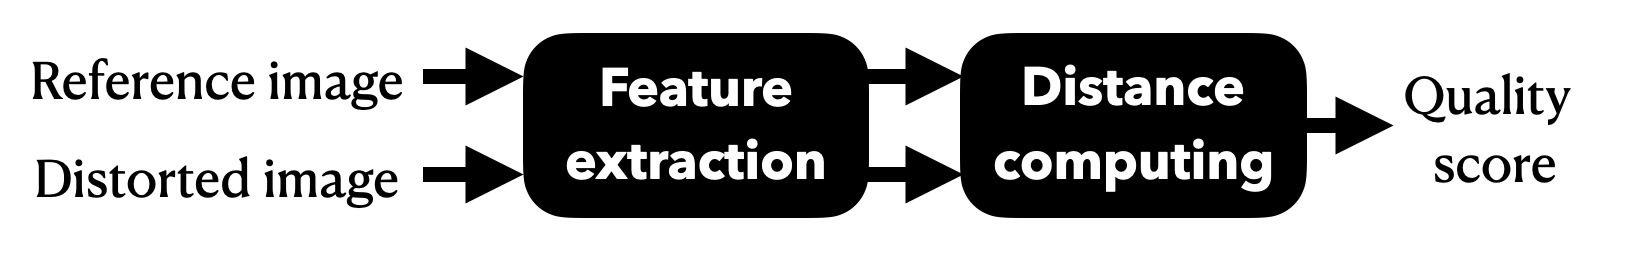
\includegraphics[keepaspectratio,width=15cm]{img/FRIQA.jpg}
    \caption{General framework of FR-IQA algorithms. Features are extracted from both images, and then the feature distance is calculated.}
    \label{fig:FRIQA}
\end{figure}
\noindent
\textbf{Full-Reference IQA} (FR-IQA) involves a comprehensive comparison between a distorted image and a reference image (see \autoref{fig:FRIQA}). Features are extracted from both images, and their differences are quantitatively analyzed to compute a quality score. While FR-IQA offers detailed assessments, it requires a reference image for every distorted image evaluated, which can limit its practicality. \par
\vspace{\baselineskip}
\begin{figure}[ht]
    \centering
    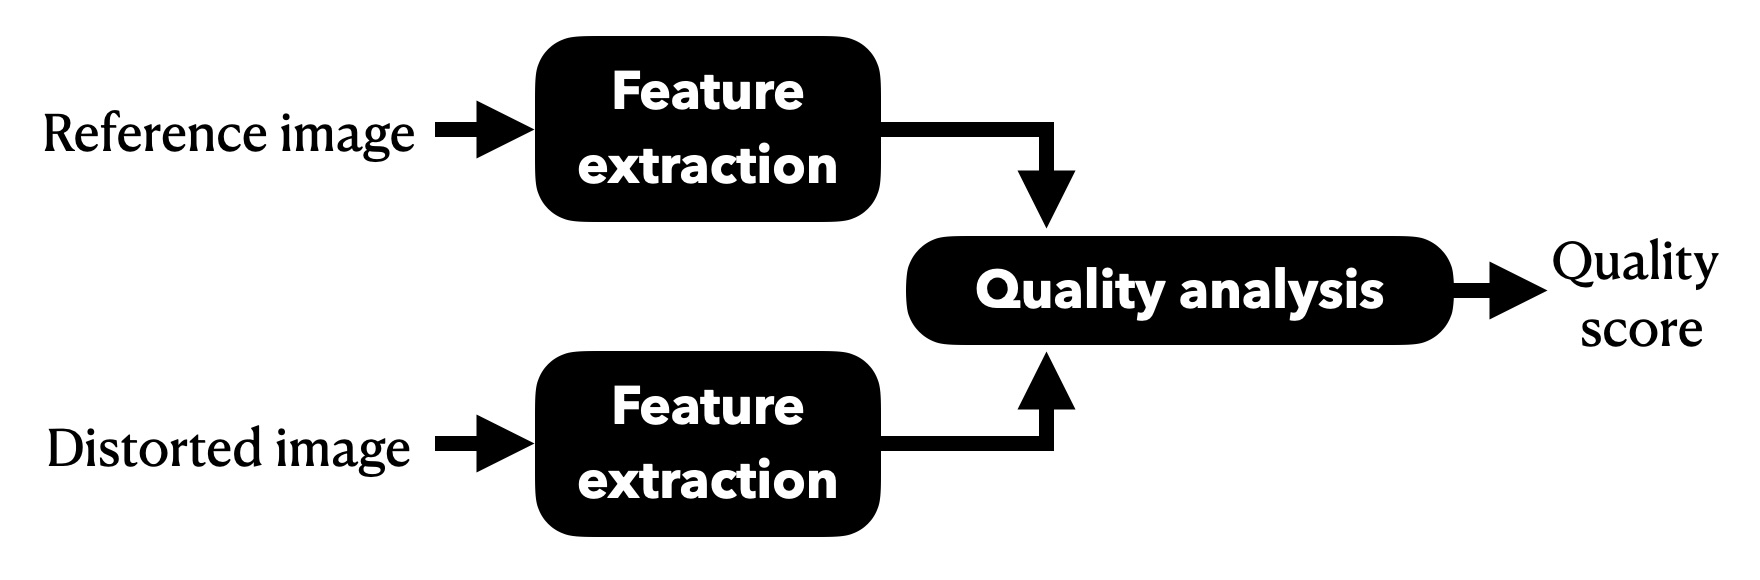
\includegraphics[keepaspectratio,width=15cm]{img/RRIQA.jpg}
    \caption{General framework of RR-IQA algorithms. Features of the reference and distorted images are extracted and used collectively to compute the quality.}
    \label{fig:RRIQA}
\end{figure}
\noindent
\textbf{Reduced-Reference IQA} (RR-IQA) operates similarly to FR-IQA but does not need the complete reference image. Instead, it uses a reduced set of features extracted from both the distorted and reference images (see \autoref{fig:RRIQA}). This method balances the exhaustive comparison of FR-IQA and the independence of NR-IQA, reducing computational demands while still providing meaningful quality assessments based on partial reference data. \par
\vspace{\baselineskip}
\noindent
Both FR-IQA and RR-IQA utilize two methods to analyze quality:
\begin{itemize}
    \item Spatial-Based Analysis: This method compares images pixel by pixel or region by region, offering straightforward interpretation and efficient computation. However, it may not fully align with how humans process images, lacking robustness in some scenarios.
    \item Transform-Based Analysis: This approach transforms images into a different domain (such as the frequency domain) that more closely mimics the human visual system. While robust, it is complex and computationally intensive.
\end{itemize}
\vspace{\baselineskip}
\begin{figure}[ht]
    \centering
    
\includegraphics[keepaspectratio,width=15cm]{img/NRIQA.jpg}
    \caption{General framework of no-reference image quality assessment algorithms.}
    \label{fig:NRIQA}
\end{figure}
\noindent
\textbf{No-Reference IQA} (NR-IQA) does not rely on any reference image. Instead, it analyzes the distorted image alone by extracting features indicative of quality (see \autoref{fig:NRIQA}). This method is particularly useful when no reference images are available, such as in many practical applications of teledermatology. NR-IQA can be tailored to address specific types of distortions or designed for general-purpose quality assessment, providing versatility across various domains. \par
\vspace{\baselineskip}
\noindent
For this thesis, the focus will be on No-Reference IQA because it is especially relevant for evaluating teledermatology images where reference images are usually not available. Since IQA measures distortions and NR-IQA can handle various types, it is important to identify the most common distortions encountered. The next subsection will discuss these distortions in detail. \par

\subsection{Common Distortions in Image Quality Assessment}
\label{sub:CommonDistortionsIQA}
mage Quality Assessment (IQA) must address various distortions that can significantly affect the perceived quality of images. Understanding these common distortions is crucial for developing effective IQA algorithms, particularly in contexts like teledermatology, where accurate image assessment is critical. Below are the common distortions typically considered in IQA, with a reference image shown first for better comparison: \par
The common distortions are:
\begin{figure}[ht]
    \centering
    \begin{subfigure}[b]{0.24\textwidth}
        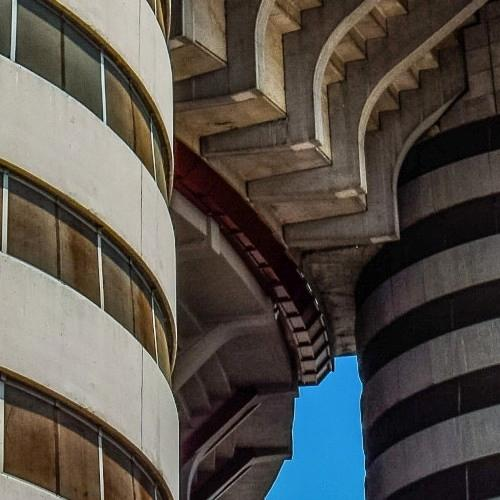
\includegraphics[width=\textwidth]{img/Original.jpg}
        \caption{Original}
    \end{subfigure}
    \hfill
    \begin{subfigure}[b]{0.24\textwidth}
        
\includegraphics[width=\textwidth]{img/Blur.jpg}
        \caption{Blur}
        \label{fig:blur}
    \end{subfigure}
    \hfill
    \begin{subfigure}[b]{0.24\textwidth}
        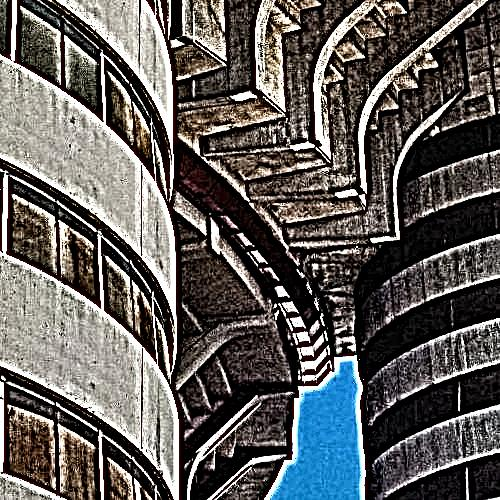
\includegraphics[width=\textwidth]{img/Sharpness.jpg}
        \caption{Sharpness}
        \label{fig:sharpness}
    \end{subfigure}
    \hfill
    \begin{subfigure}[b]{0.24\textwidth}
        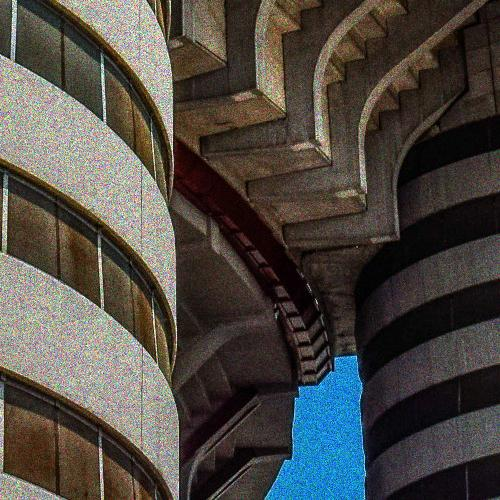
\includegraphics[width=\textwidth]{img/Noise.jpg}
        \caption{Noise}
        \label{fig:noise}
    \end{subfigure} 

    \begin{subfigure}[b]{0.24\textwidth}
        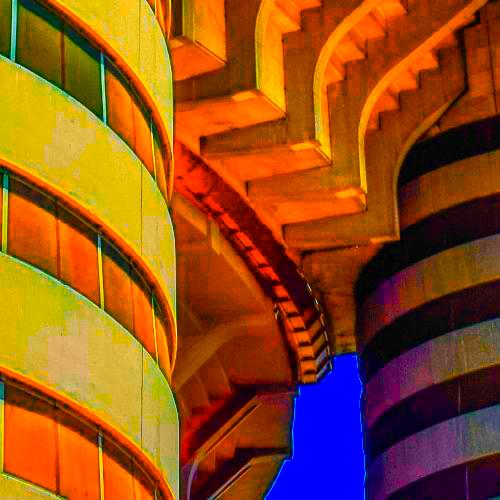
\includegraphics[width=\textwidth]{img/ColorAccuracy.jpg}
        \caption{Color Accuracy}
        \label{fig:color_accuracy}
    \end{subfigure}
    \hfill
    \begin{subfigure}[b]{0.24\textwidth}
        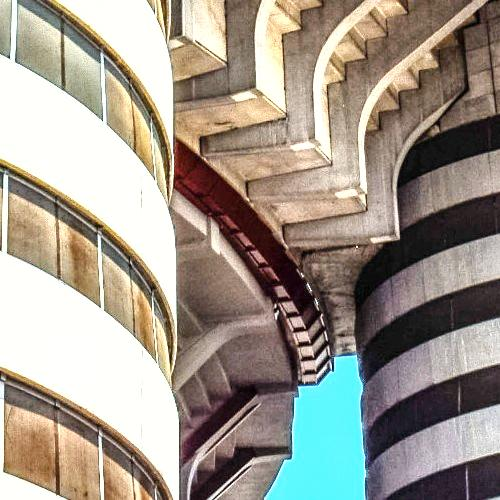
\includegraphics[width=\textwidth]{img/BrightnessContrast.jpg}
        \caption{Brightness \& Contrast}
        \label{fig:brightness_contrast}
    \end{subfigure}
    \hfill
    \begin{subfigure}[b]{0.24\textwidth}
        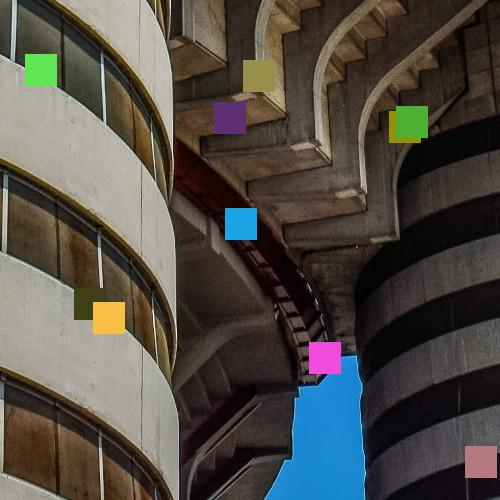
\includegraphics[width=\textwidth]{img/Artifacts.jpg}
        \caption{Artifacts}
        \label{fig:artifacts}
    \end{subfigure}
    \hfill
    \begin{subfigure}[b]{0.24\textwidth}
        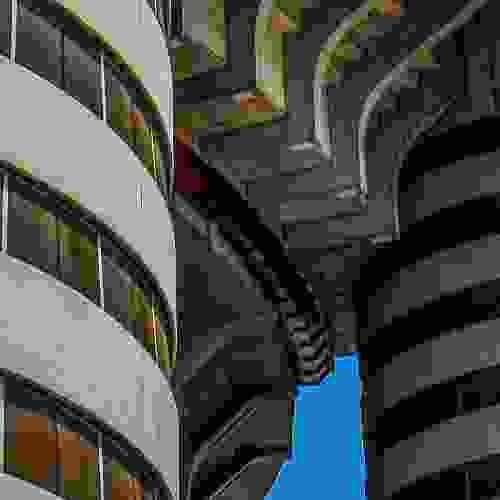
\includegraphics[width=\textwidth]{img/Compression.jpg}
        \caption{Compression}
        \label{fig:compression}
    \end{subfigure}
    \caption{Examples of Common Distortions in Images. (adapted from \autocite{ARNIQA})}
    \label{fig:distortions}
\end{figure}
\begin{enumerate}
    \item \textbf{Blur}: Blurred images lack sharpness and clarity, often resulting from motion during capturing, incorrect focus settings, or imperfections in the camera lens. See \autoref{fig:blur} for an example of a blurred image.
    \item \textbf{Sharpness}: Sharpness refers to how well-defined the edges and fine details in an image appear. High sharpness indicates clear, crisp images, while low sharpness makes an image look soft and unclear. See \autoref{fig:sharpness} for an example of a sharpened image.
    \item \textbf{Noise}: Noise appears as random variations in brightness or color and is often due to the limitations of the camera’s sensor, particularly under low light conditions or at high ISO settings. See \autoref{fig:noise} for an example of a noisy image.
    \item \textbf{Color Accuracy}:  Color accuracy refers to how faithfully colors are reproduced in an image. Distortions in color accuracy can lead to inaccurate or unrealistic color representation. See \autoref{fig:color_accuracy} for an example of a color-distorted image.
    \item \textbf{Brightness \& Contrast}: Brightness is the overall light level of an image, while contrast refers to the range between its darkest and lightest areas. Proper balance of both is crucial for maintaining image visibility and detail. Excessive or insufficient brightness and contrast can make an image unusable for detailed analysis. See \autoref{fig:brightness_contrast} for an example of an image with altered brightness.
    \item \textbf{Artifacts}: Artifacts are unwanted visual anomalies introduced during image acquisition or processing, such as halos, or jagged edges. See \autoref{fig:artifacts} for an example of an image with artifacts.
    \item \textbf{Compression}: When images are compressed to reduce file size, this often results in lost detail and visible quality degradation. See \autoref{fig:compression} for an example of a compressed image.
\end{enumerate}
Each type of distortion affects the visual quality and perceived accuracy of images, influencing the effectiveness of IQA methodologies in assessing image quality. Understanding these distortions is essential for developing robust quality assessment algorithms and improving image clarity in various applications, including teledermatology. \par

\subsection{Benchmark Datasets for IQA}
\label{sub:BenchmarkDatasetsIQA}
Benchmark datasets play a vital role in advancing Image Quality Assessment (IQA). They provide standardized and diverse image sets with known distortions and corresponding quality annotations, helping researchers evaluate and improve IQA algorithms. These annotations, often in the form of Mean Opinion Score (MOS) and Differential Mean Opinion Score (DMOS), serve as benchmarks for algorithm performance. \par
\vspace{\baselineskip}
\noindent
\textbf{Mean Opinion Score (MOS)} is calculated by averaging ratings from human observers who judge the quality of images on a predefined scale. This score reflects the overall perceptual quality as seen by typical viewers and is widely used to compare the performance of different IQA methods against human visual judgment. \par
\vspace{\baselineskip}
\noindent
\textbf{Differential Mean Opinion Score (DMOS)}, on the other hand, is derived from MOS and measures the perceived difference in quality between a reference image and a distorted version. This score is particularly useful for understanding the impact of specific distortions on image quality. \par
\vspace{\baselineskip}
\noindent
These datasets enable researchers to thoroughly test the robustness, accuracy, and generalization capabilities of different IQA methods. They also help in developing new algorithms by providing reliable quality scores, which are essential for ensuring reproducible. \par
\noindent
An overview of IQA databases is provided in \autoref{tab:iqa_databases}, and more detailed descriptions can be found in \autoref{ch:Dataset}.

\begin{table*}[!t]
    \centering
    \caption{An overview of IQA databases}
    \label{tab:iqa_databases}
    \renewcommand{\arraystretch}{1.5}
    \resizebox{\textwidth}{!}{ % Resize table to fit within the text width
    \begin{tabular}{p{2.3cm} p{2cm} c c c p{3.5cm} c  p{2.3cm} c}
    \toprule
        Category & Database & Year & \#Ref. & \#Dist. & \#Dist. Type & \#Dist. Level & Resolution Type & Ground-truth \\
        \hline
        \multirow{8}{*}{General} 
        & LIVE & 2004 & 30 & 779 & JPEG, JP2K, WN, GB, FF& 5 or 4 & 768 $\times$ 512 & DMOS \\
        & TID2008 & 2008 & 25 & 1700 & 17 \footnote{See detailed types on database page: \url{https://www.ponomarenko.info/tid2008.htm}} & 4 & 512 $\times$ 384 & MOS \\
        & TID2013 & 2013 & 25 & 3000 & 24 \footnote{See detailed types on database page: \url{https://www.ponomarenko.info/tid2013.htm}} & 5 & 512 $\times$ 384 & MOS \\
        & CSIQ & 2009 & 30 & 866 & JPEG, JP2K, WN, GB, APGN,  GCD & 5 or 4 & 512 $\times$ 512 & DMOS \\
        & A57 & 2007 & 3 & 54 & DWT, AGWN, JPEG, JP2K, JP2K-DCQ, GB& 3 & 512 $\times$ 512 & MOS \\
        & WED & 2017 & 4744 & 94880 & JPEG, JP2K, GB, WN& 5 & - & - \\
        & KADID-10k & 2019& 81& 10125& 25 \footnote{See detailed types on database page: \url{https://database.mmsp-kn.de/kadid-10k-database.html}} & 5& 512 $\times$ 384 & DMOS\\
        & KADIS-700k & 2020& 140000& 700000& 25 \footnote{See detailed types on database page: \url{https://database.mmsp-kn.de/kadid-10k-database.html}} & 5& 512 $\times$ 384 & DMOS\\
        \hline
        \multirow{3}{*}{Multiple Dist.} 
        & LIVEMD & 2012 & 15 & 405 & GB followed by JPEG, GB followed by WN& - & 1280 $\times$ 720 & DMOS \\
        & MDID2013 & 2013 & 12 & 324 & corrupted successively by GB, WN, and JPEG& - & 768 $\times$ 512 or 1280 $\times$ 720 & DMOS \\
        & MDID2016 & 2016 & 20 & 1600 & GB or CC first, JPEG or JP2K second and WN last& - & 512 $\times$ 384 & MOS \\
        \hline
        \multirow{4}{*}{Screen content} 
        & SIQAD & 2014 & 20 & 980 & WN, GB, CC, JPEG, JP2K, MB, LSBC& 7 & 700 $\times$ 700 & DMOS \\
        & SCIQ & 2017 & 40 & 1800 & WN, GB, MB, CC, JPEG, JP2K, CSC, CQD& 5 & 1280 $\times$ 720 & MOS \\
        & CCT & 2017 & 72 & 1320 & HEVC and HEVC-SCC coding& 11 & 1280 $\times$ 720 to 1920 $\times$ 1080 & MOS \\
        & HSNID & 2019 & 20 & 600 & WN, GB, MB, CC, JPEG, JP2K& 5 &  - & MOS \\
        \hline
        \multirow{2}{*}{Authentic Dist.} 
        & LIVE Wild & 2016 & 0 & 1162 & - & - & 500 $\times$ 500 & MOS \\
        & CID2013 & 2015 & 0 & 480 & - & - & 1600 $\times$ 1200 & MOS \\
    \bottomrule
    \end{tabular}
    }
    \raggedright
    \scalebox{0.59}{
    \begin{tabular}{l}
        Note: \#Ref.: Total number of pristine images. \quad \#Dist.: Total number of distorted images. \quad AGWN: Additive Gaussian white noise. \quad WN: White noise.\\
        \quad  \quad  \quad APGN: Additive pink Gaussian noise. \quad CC: Contrast change. \quad CSC: Color saturation change. \quad CQD: Color quantization with dithering.\\
        \quad  \quad  \quad DWT: Quantization of the LH subbands of a 5-level DWT. \quad FF: Simulated fast fading Rayleigh channel. \quad GB: Gaussian blur. \quad MB: Motion blur.\\
        \quad  \quad  \quad GCD: Global contrast decrements. \quad HEVC-SCC: Screen content coding extension of high efficiency video coding. \quad JPEG: JPEG compression. \\
        \quad  \quad  \quad JP2K: JPEG2000 compression. \quad JP2K-DCQ: JPEG-2000 compression with DCQ. \quad LSBC: Layer segmentation based compression.
    \end{tabular}
    }
\end{table*}


\subsection{State-of-the-Art in Image Quality Assessment}
\label{sub:SOTA_IQA}
The current state-of-the-art in Image Quality Assessment (IQA) is ARNIQA \autocite{ARNIQA} , with version 2 released on November 4, 2023. ARNIQA (leArning distoRtion maNifold for Image Quality Assessment) represents a major advancement in No-Reference Image Quality Assessment (NR-IQA). This technology aims to measure image quality based on human perception, even without a reference image. This capability is crucial in fields like teledermatology, where the quality of images directly impacts diagnostic accuracy. \par
\vspace{\baselineskip}
\noindent
\textbf{Overview}: ARNIQA is developed using a self-supervised learning approach. It learns a comprehensive model of all possible image distortions, focusing on the types and quality of distortions rather than the content of the images themselves. This makes it highly adaptable across various domains where image content can differ significantly. \par
\vspace{\baselineskip}
\noindent
\textbf{Key Features}:
\begin{figure}[ht]
    \centering
    
\includegraphics[keepaspectratio,width=15cm]{img/method_SimCLR.jpg}
    \caption{Overview of the training strategy for ARNIQA. Two pristine images are cropped and equally degraded. The model maximizes the similarity of their embeddings while minimizing the similarity to embeddings from degraded crops of half-scale versions of the original images. This process creates hard negative examples by introducing downsample distortion, demonstrating how original and half-scale degraded crops differ despite identical degradation. \autocite{ARNIQA}.}
    \label{fig:SimCLR}
\end{figure}
\begin{enumerate}
    \item Image Degradation Model: ARNIQA can synthetically degrade images through up to 1.9 billion distinct degradation patterns. This model can apply up to seven different types of distortions in one sequence, covering a wide range of real-world scenarios. Training with such diverse distortions ensures that ARNIQA can accurately assess image quality across various conditions and avoid the need for large labeled datasets.
    \item SimCLR Framework: At the core of ARNIQA is the SimCLR (Simple Framework for Contrastive Learning) framework. This framework enables the model to learn meaningful representations of image quality by comparing different versions of the same image and focusing on their similarities and differences. SimCLR constructs positive pairs by applying the same distortion settings to two different images, ensuring that the model concentrates on the distortions rather than the content. To further enhance the model’s discriminative capability, SimCLR introduces subtle variations by downsampling images before cropping and applying distortions, creating hard negative examples. These examples help the model differentiate between similar-looking images with different types of degradation. By using this approach, the SimCLR framework ensures that ARNIQA effectively learns to recognize and assess various distortions, enhancing its ability to provide accurate image quality assessments (see \autoref{fig:SimCLR}).
    \item Linear Regressor: A Linear Regressor maps the features learned by SimCLR to qualtiy score ranging from 0 to 1. This score reflects the relative quality of the image based on the distortions present.
\end{enumerate}
\vspace{\baselineskip}
\noindent
\textbf{Training Strategy}: ARNIQA’s training strategy involves two main phases: \par
\begin{enumerate}
    \item Encoder Pre-training: The model is first trained on a large set of unlabeled images that are synthetically degraded. This helps the encoder learn features related to different types and levels of image degradation.
    \item Regressor Training:In the second phase, a specific regressor is trained using the Mean Opinion Scores (MOS) of images. This step translates the learned features into actual quality scores.
\end{enumerate}
\vspace{\baselineskip}
\noindent
\textbf{Evaluation Metrics}: ARNIQA uses SRCC (Spearman’s Rank Order Correlation Coefficient) and PLCC (Pearson Linear Correlation Coefficient) to evaluate its performance. These metrics measure how well the model's predictions match the actual image quality rankings and scores. \par
\vspace{\baselineskip}
\noindent
SRCC checks how well the predicted rankings of image quality match the actual rankings. It is calculated as: \par
\begin{equation}
    SRCC = 1 - \frac{6 \sum_{i=1}^n (d_i^2)}{n(n^2 - 1)}
\end{equation}
\noindent
where, \newline
$n: \text{Number of images} \\ d_i: \text{Difference in ranks between predicted and actual scores for image } i$ \par
\vspace{\baselineskip}
\noindent
An SRCC of 1 means perfect rank correlation, and -1 means perfect negative correlation. \par
\vspace{\baselineskip}
\noindent
PLCC measures the linear relationship between the predicted and actual quality scores. It is calculated as: \par
\begin{equation}
    PLCC = \frac{\sum_{i=1}^n (P_i - \bar{P})(A_i - \bar{A})}{\sqrt{\sum_{i=1}^n (P_i - \bar{P})^2 \sum_{i=1}^n (A_i - \bar{A})^2}}
\end{equation}
\noindent
where, \newline
$n: \text{Number of images} \\ P_i: \text{Predicted score for image } i \\ A_i: \text{Actual score for image } i \\ \bar{P}: \text{Average predicted score} \\ \bar{A}: \text{Average actual score}$ \par
\vspace{\baselineskip}
\noindent
A PLCC of 1 means a perfect positive linear relationship, and -1 means a perfect negative linear relationship. \par
\vspace{\baselineskip}
\noindent
\textbf{Advantages}: ARNIQA achieves high performance with only up to 0.5\% of the data required by other methods, thanks to its focus on distortion patterns rather than image content. It provides reliable and consistent quality assessments across a wide range of distortions and severities, demonstrating its robustness. Additionally, ARNIQA is particularly suitable for teledermatology as it can handle varying image quality resulting from different lighting conditions, camera quality, and patient handling. \par

\subsection{Challenges and Opportunities in Image Quality Assessment}
\label{sub:ChallengesOpportunitiesIQA}
One major challenge in IQA is that assessing image quality can be very subjective. Different people can have different opinions on what looks good or bad, making it hard to create standard measures. This is especially important in teledermatology, where the quality of images directly affects medical diagnoses. Another challenge is that images can have many types of problems, like blurring, noise, compression artifacts, and color issues. Each problem affects the image in a different way, and it’s tough to develop IQA methods that can handle all these issues accurately. Additionally, in many real-world applications, including teledermatology, we often don’t have high-quality reference images to compare against. This makes it difficult to evaluate the quality of distorted images. Therefore, developing methods that don’t need reference images (No-Reference IQA) is essential.\par
\vspace{\baselineskip}
\noindent
A big opportunity in IQA is the advancement of self-supervised learning techniques. These methods, like those used in ARNIQA, allow models to learn from large amounts of data without needing a lot of labeled examples. This approach saves time and money because it reduces the need for manually labeled data. It also makes it possible to develop high-quality IQA models that can work well even without reference images. \par
\vspace{\baselineskip}
\noindent
By addressing these challenges and leveraging the opportunities, we can significantly improve how we assess image quality. \par
\clearpage

\section{Teledermatology}
\label{sec:Teledermatology}
This section covers teledermatology and highlights the importance of image quality in remote skin assessments. We will start by explaining what teledermatology is and then discuss why having high-quality images is crucial for accurate diagnoses and treatment. \par
\vspace{\baselineskip}
\noindent
We’ll also look at the quality standards needed for teledermatology images and review public datasets available for research. Next, we’ll briefly examine different methods used to assess image quality in teledermatology, based on previous studies. Finally, we’ll explore the challenges and opportunities in the field, focusing on how to improve image quality assessment. This approach will help us understand the current state of teledermatology and find ways to enhance it.\par

\subsection{Introduction to Teledermatology}
\label{sub:IntroductionTeledermatology}
Teledermatology is a branch of telemedicine that allows dermatologists to provide remote consultations and treatment using telecommunications technology. This is especially helpful for patients in remote areas, ensuring they get timely and effective skin care. There are two main methods used in teledermatology: real-time (synchronous) and store-and-forward (asynchronous).\par
\vspace{\baselineskip}
\noindent
\textbf{Real-time} teledermatology involves live video consultations between the dermatologist and the patient. This allows for immediate interaction and feedback, making it useful for urgent cases. However, it requires both the patient and the dermatologist to be available at the same time, which can be a limitation. \par
\vspace{\baselineskip}
\noindent
\textbf{Store-and-forward} teledermatology involves sending medical information, including images and patient history, to dermatologists who review it later. This method offers more flexibility since it doesn’t require the patient and dermatologist to be available simultaneously \autocite{SaF}. \autoref{fig:TD_workflow} shows the process of a teledermatology consultation, from the patient taking pictures of their skin condition to receiving a detailed medical report. Each step highlights the importance of image quality for accurate diagnosis and effective patient care.\par
\vspace{\baselineskip}
\noindent
High-quality images are crucial in teledermatology because they directly impact the accuracy of remote diagnoses. Poor image quality can lead to incorrect diagnoses or delayed treatment, reducing the benefits of teledermatology. Therefore, ensuring that images meet specific quality standards is essential for successful teledermatology services.

\subsection{Quality Criteria for Teledermatology Images}
\label{sub:QualityCriteriaTeledermatology}
High-quality images are crucial in teledermatology to ensure accurate diagnoses and effective patient care. The International Skin Imaging Collaboration (ISIC)  has set guidelines for standardizing images. Out of nine recommended criteria, we will focus on seven key criteria that directly impact image quality. The other two, “Scale and Measurement” and “Image Storage,” are not relevant because they are not directly related to image quality in teledermatology. “Scale and Measurement” is less important in this context, and “Image Storage” deals more with regulations than with image quality \autocite{TDCriteria}. \par
\vspace{\baselineskip}
\noindent
Here are the seven key criteria for teledermatology images, illustrated in \autoref{fig:quality_criteria}, along with recommendations on how to meet each criteria:
\vspace{\baselineskip}
\begin{figure}[ht]
    \centering
    \begin{subfigure}[b]{0.24\textwidth}
        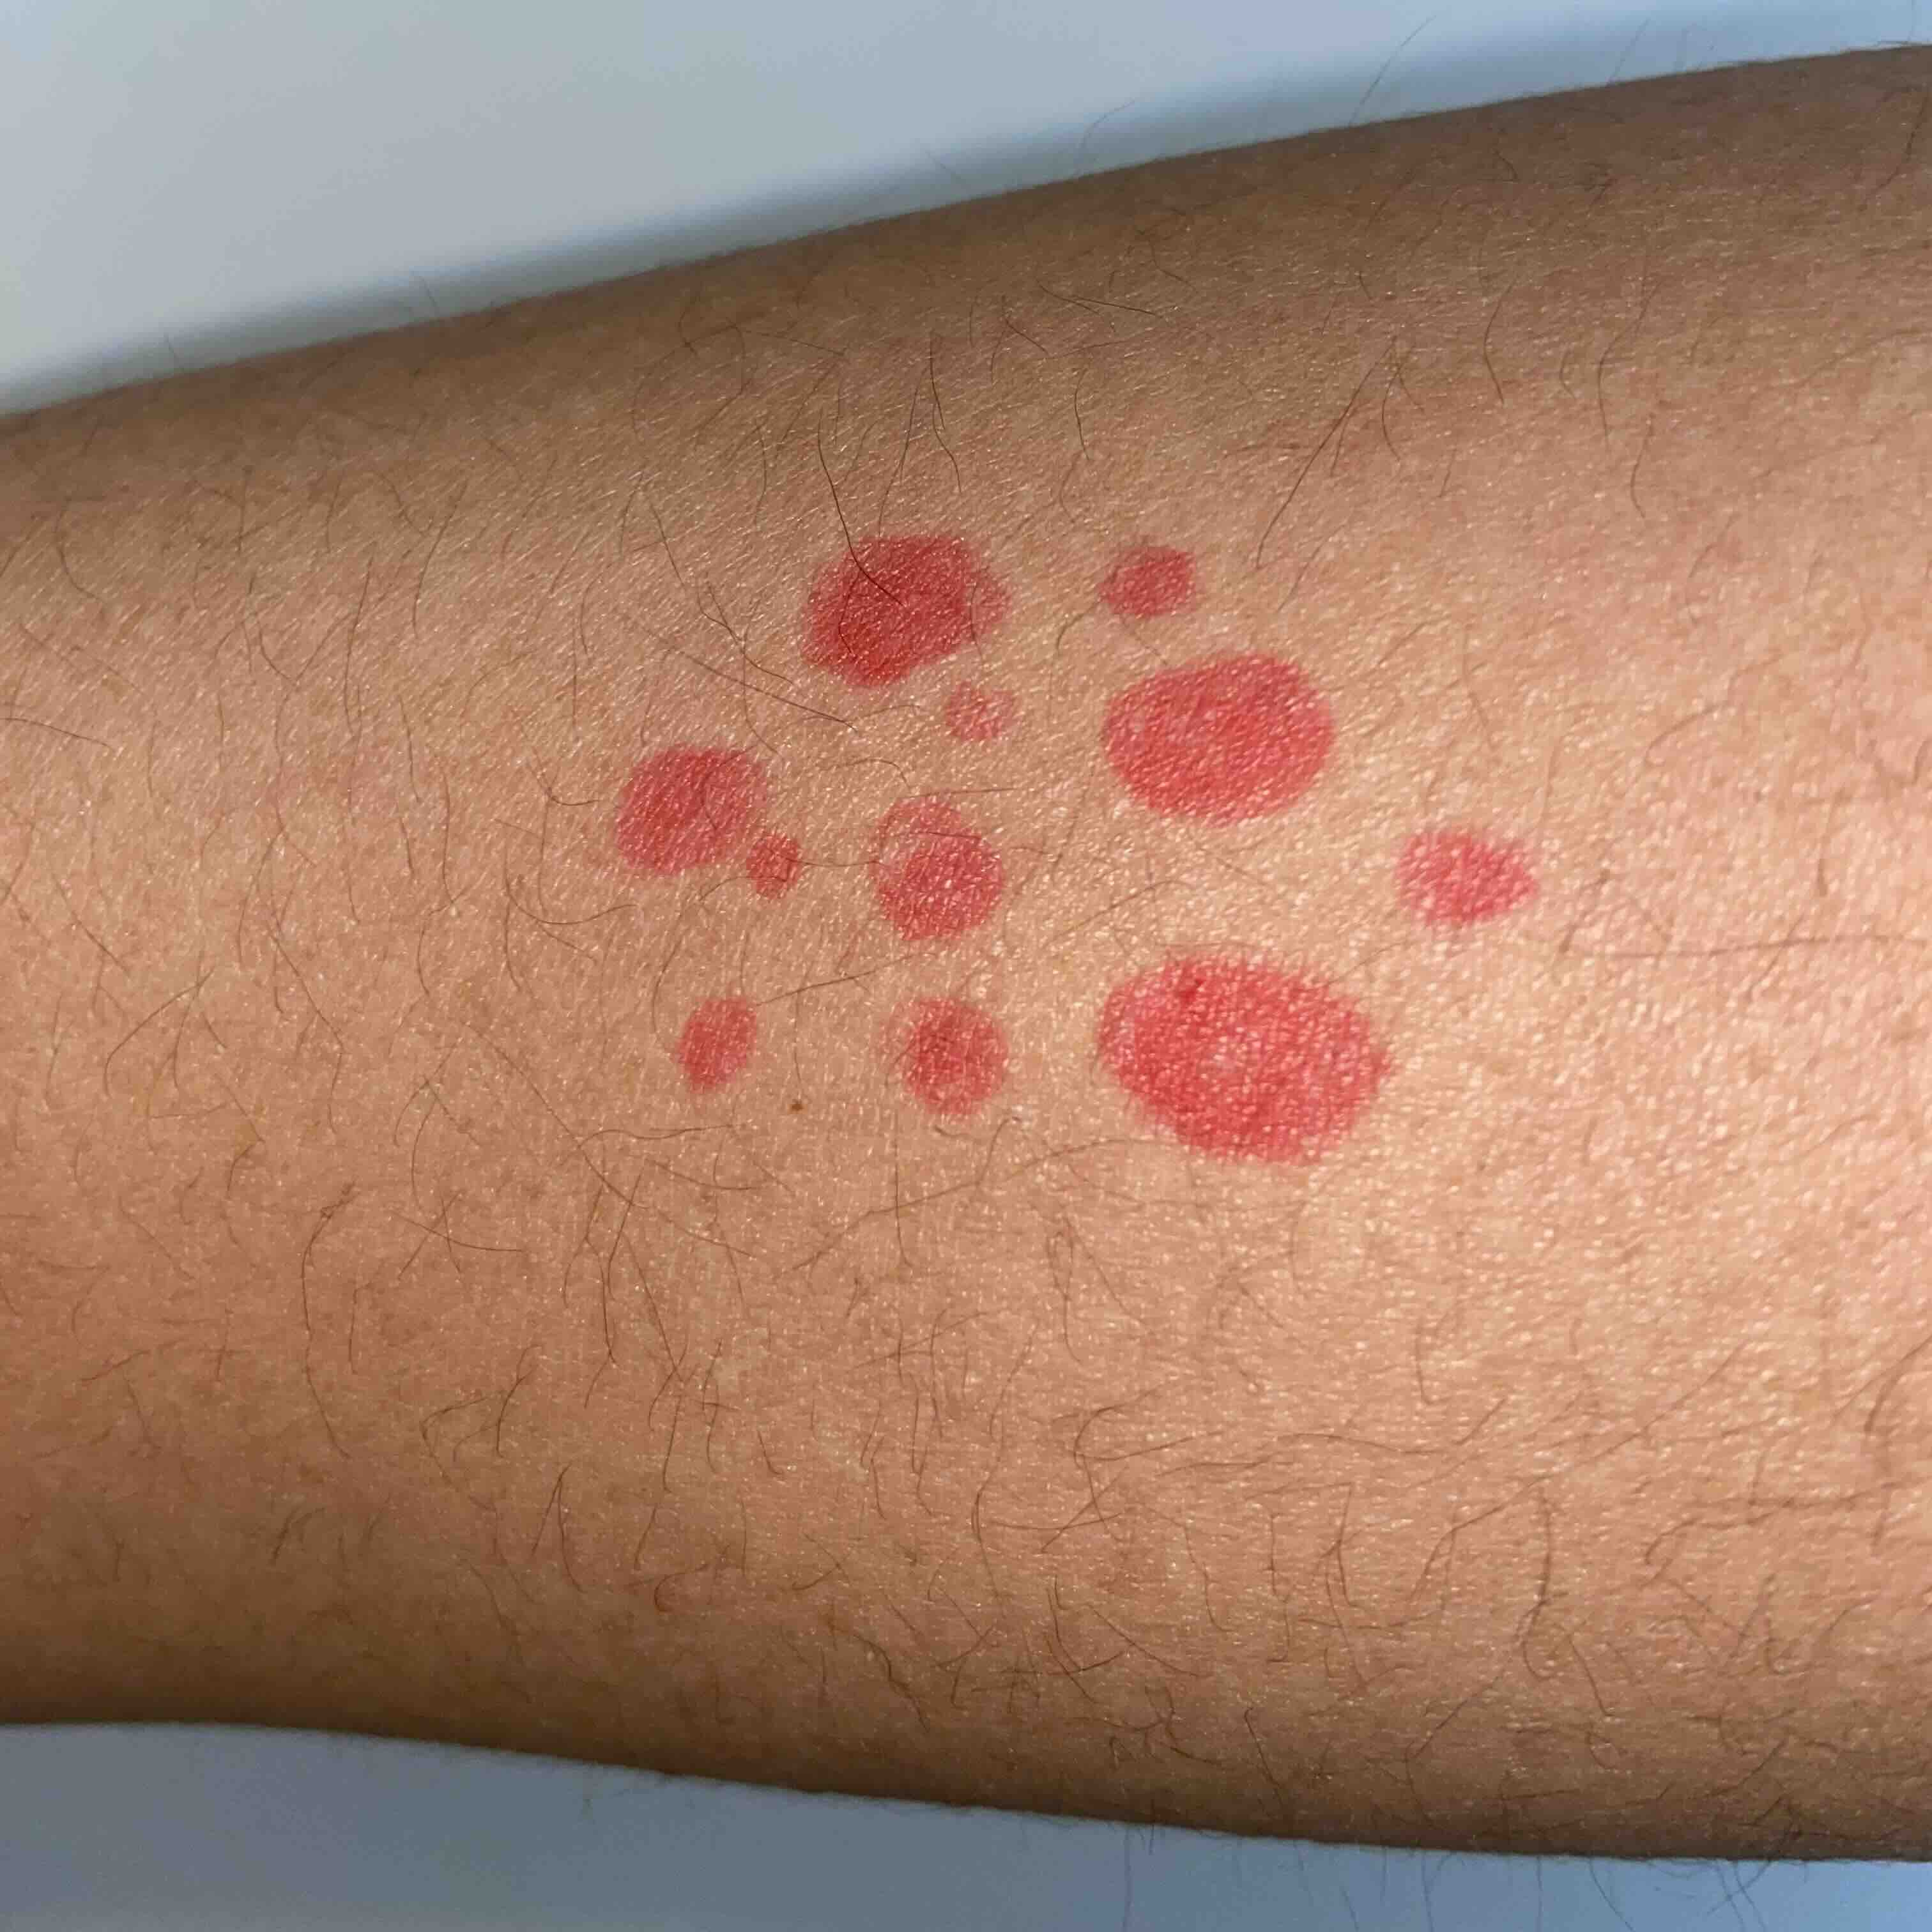
\includegraphics[width=\textwidth]{img/Reference.jpg}
        \caption{Good Quality}
    \end{subfigure}
    \hfill
    \begin{subfigure}[b]{0.24\textwidth}
        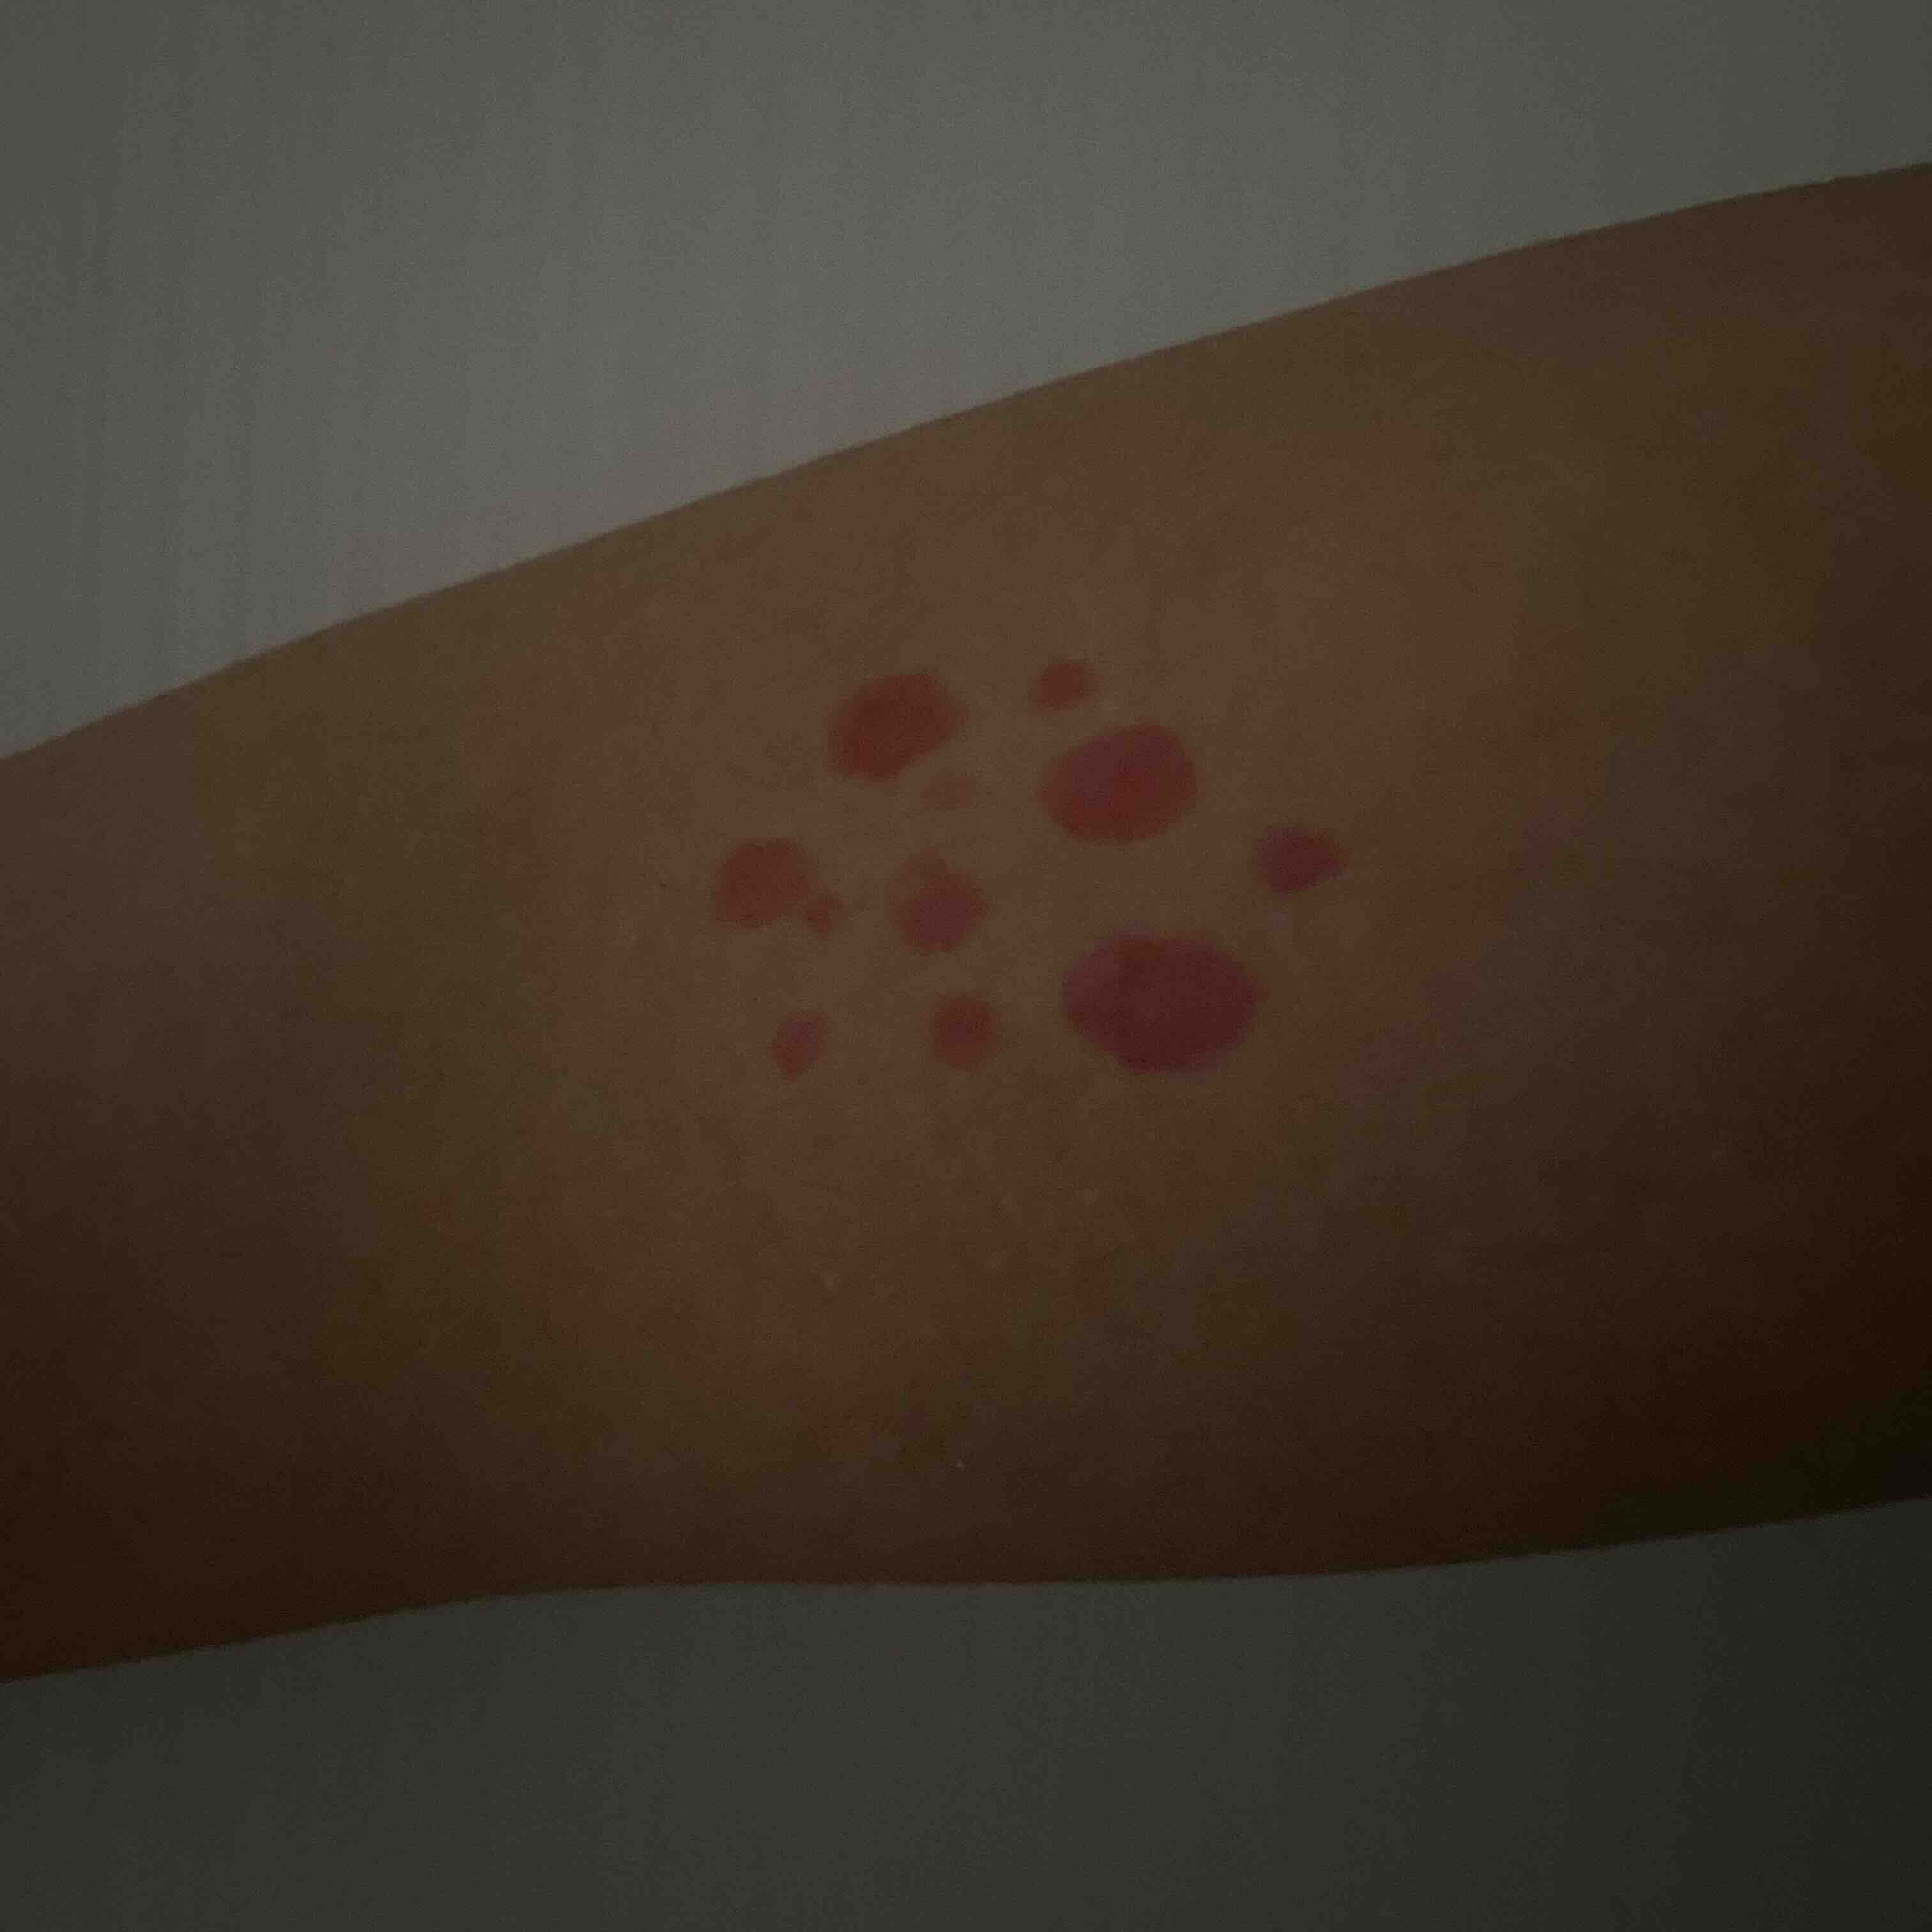
\includegraphics[width=\textwidth]{img/Lighting.jpg}
        \caption{Lighting}
        \label{fig:lighting}
    \end{subfigure}
    \hfill
    \begin{subfigure}[b]{0.24\textwidth}
        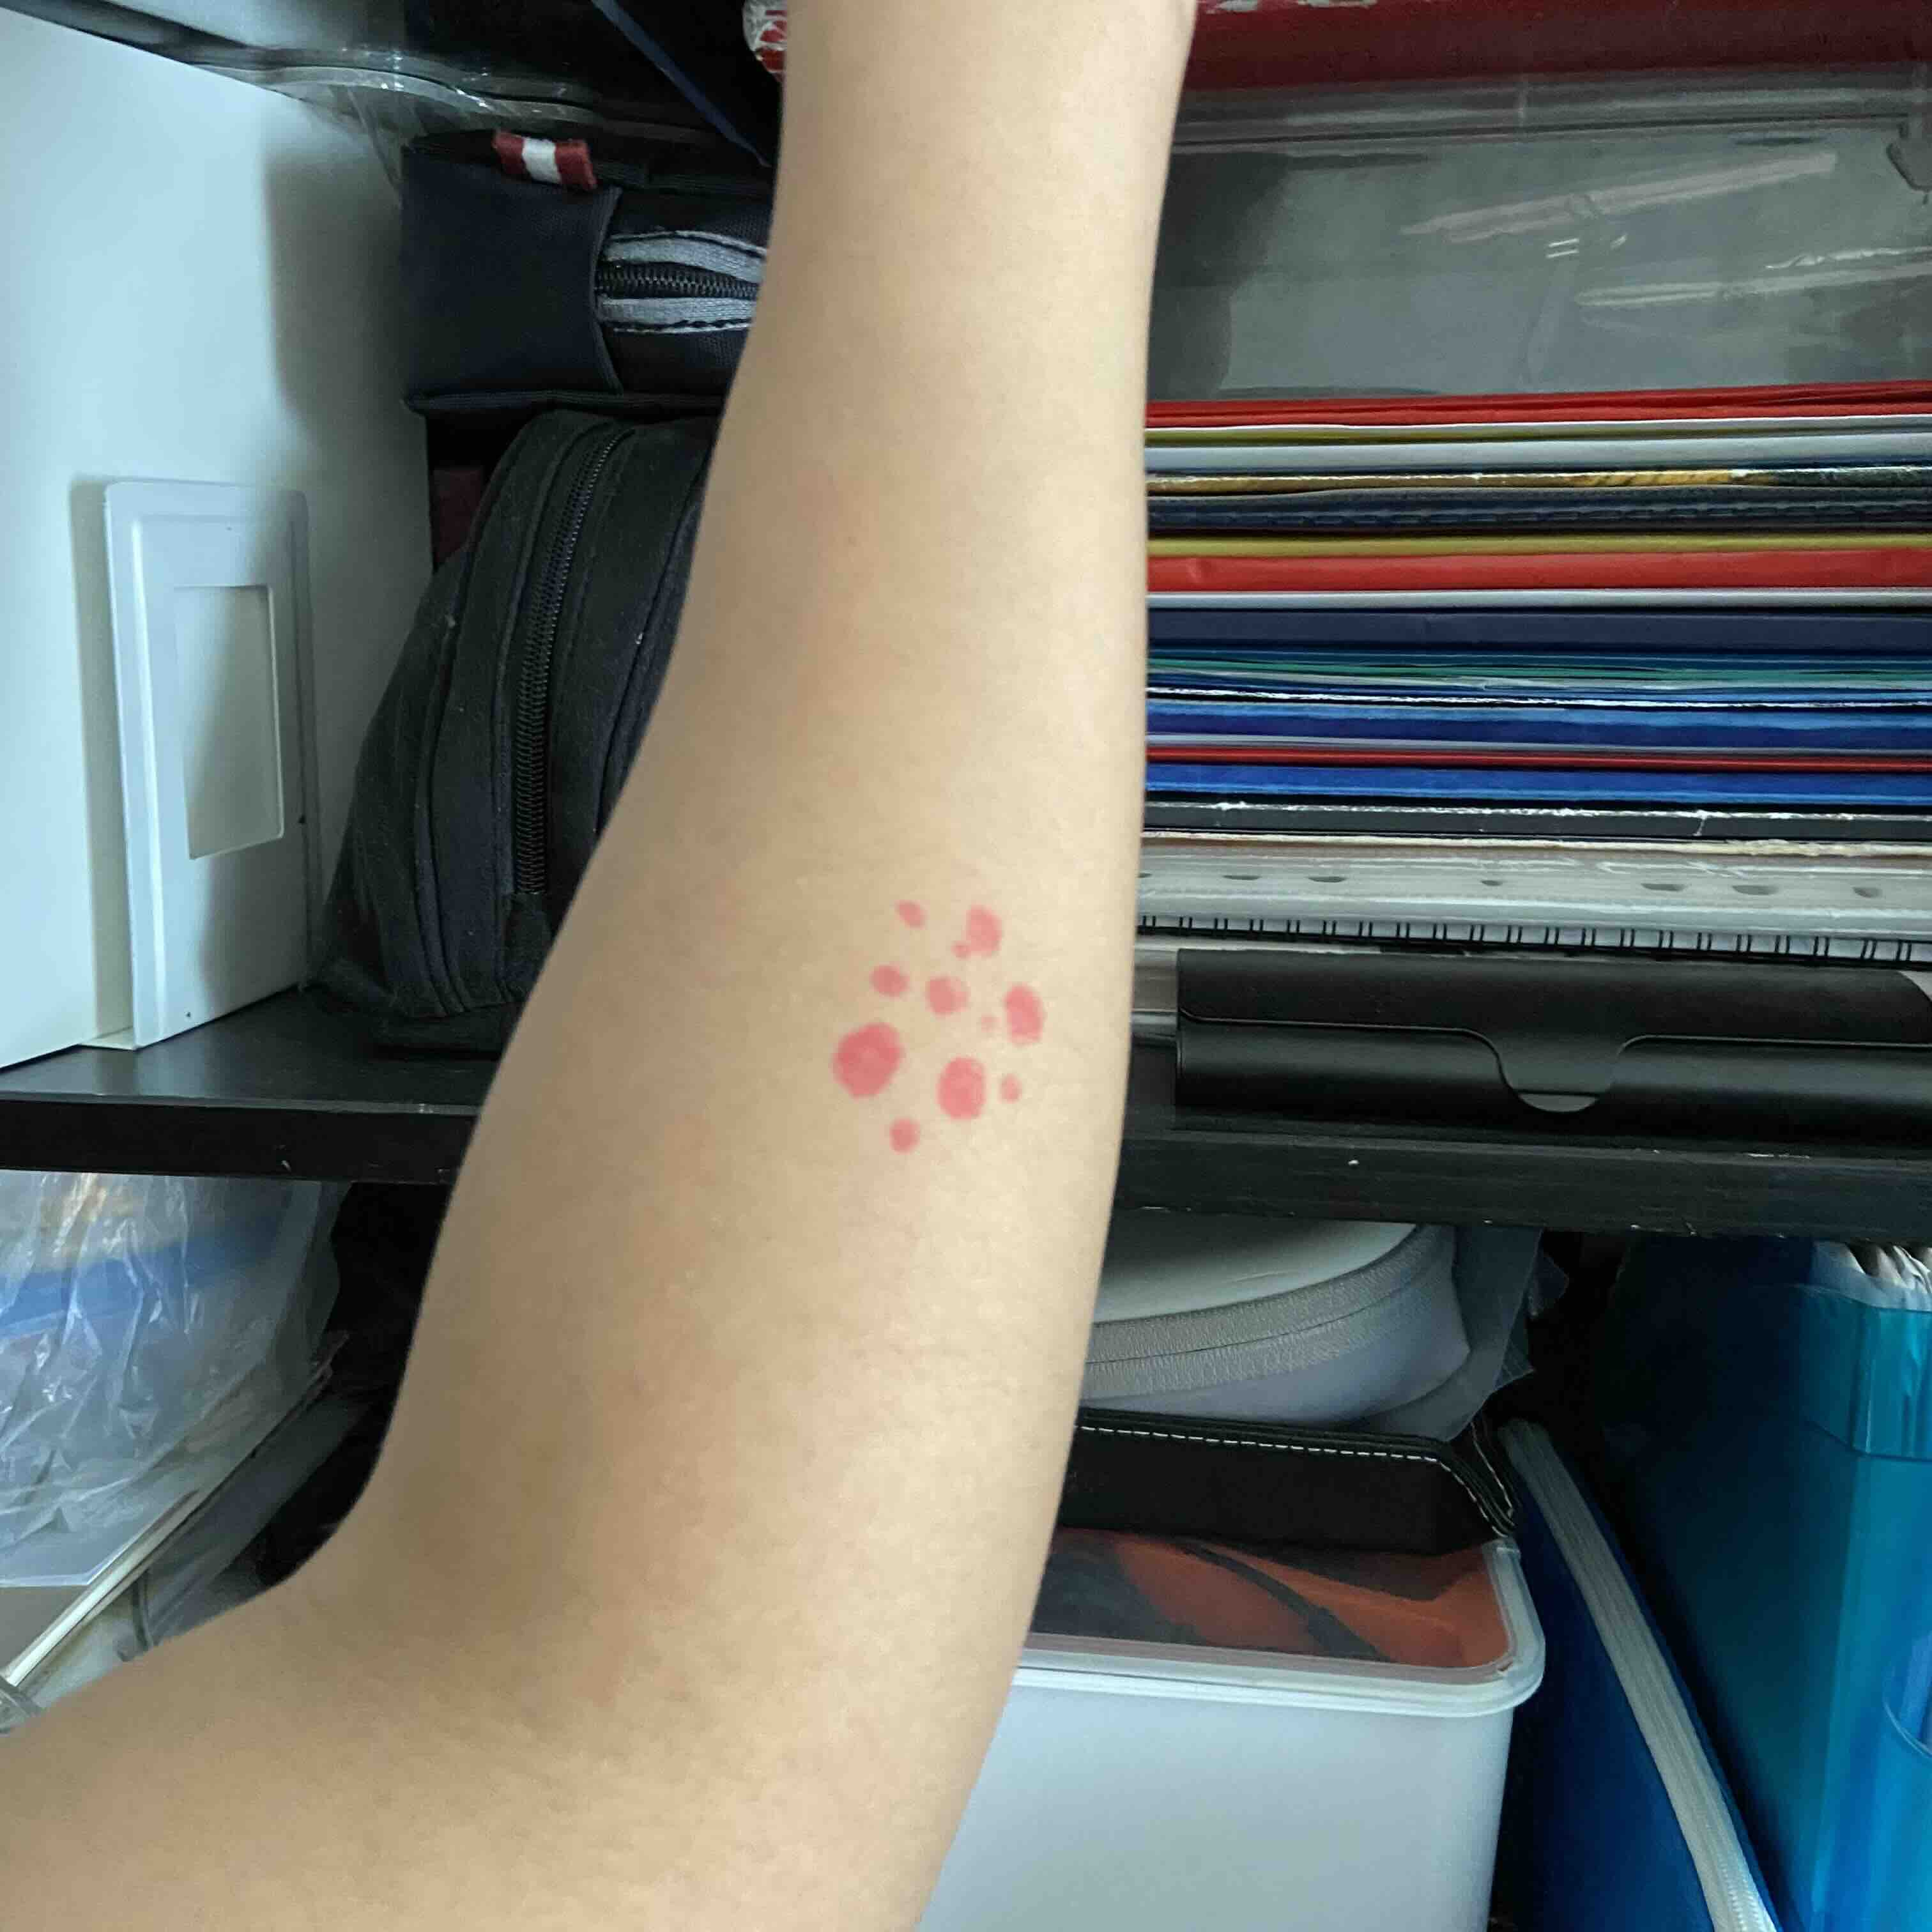
\includegraphics[width=\textwidth]{img/Background.jpg}
        \caption{Background}
        \label{fig:background}
    \end{subfigure}
    \hfill
    \begin{subfigure}[b]{0.24\textwidth}
        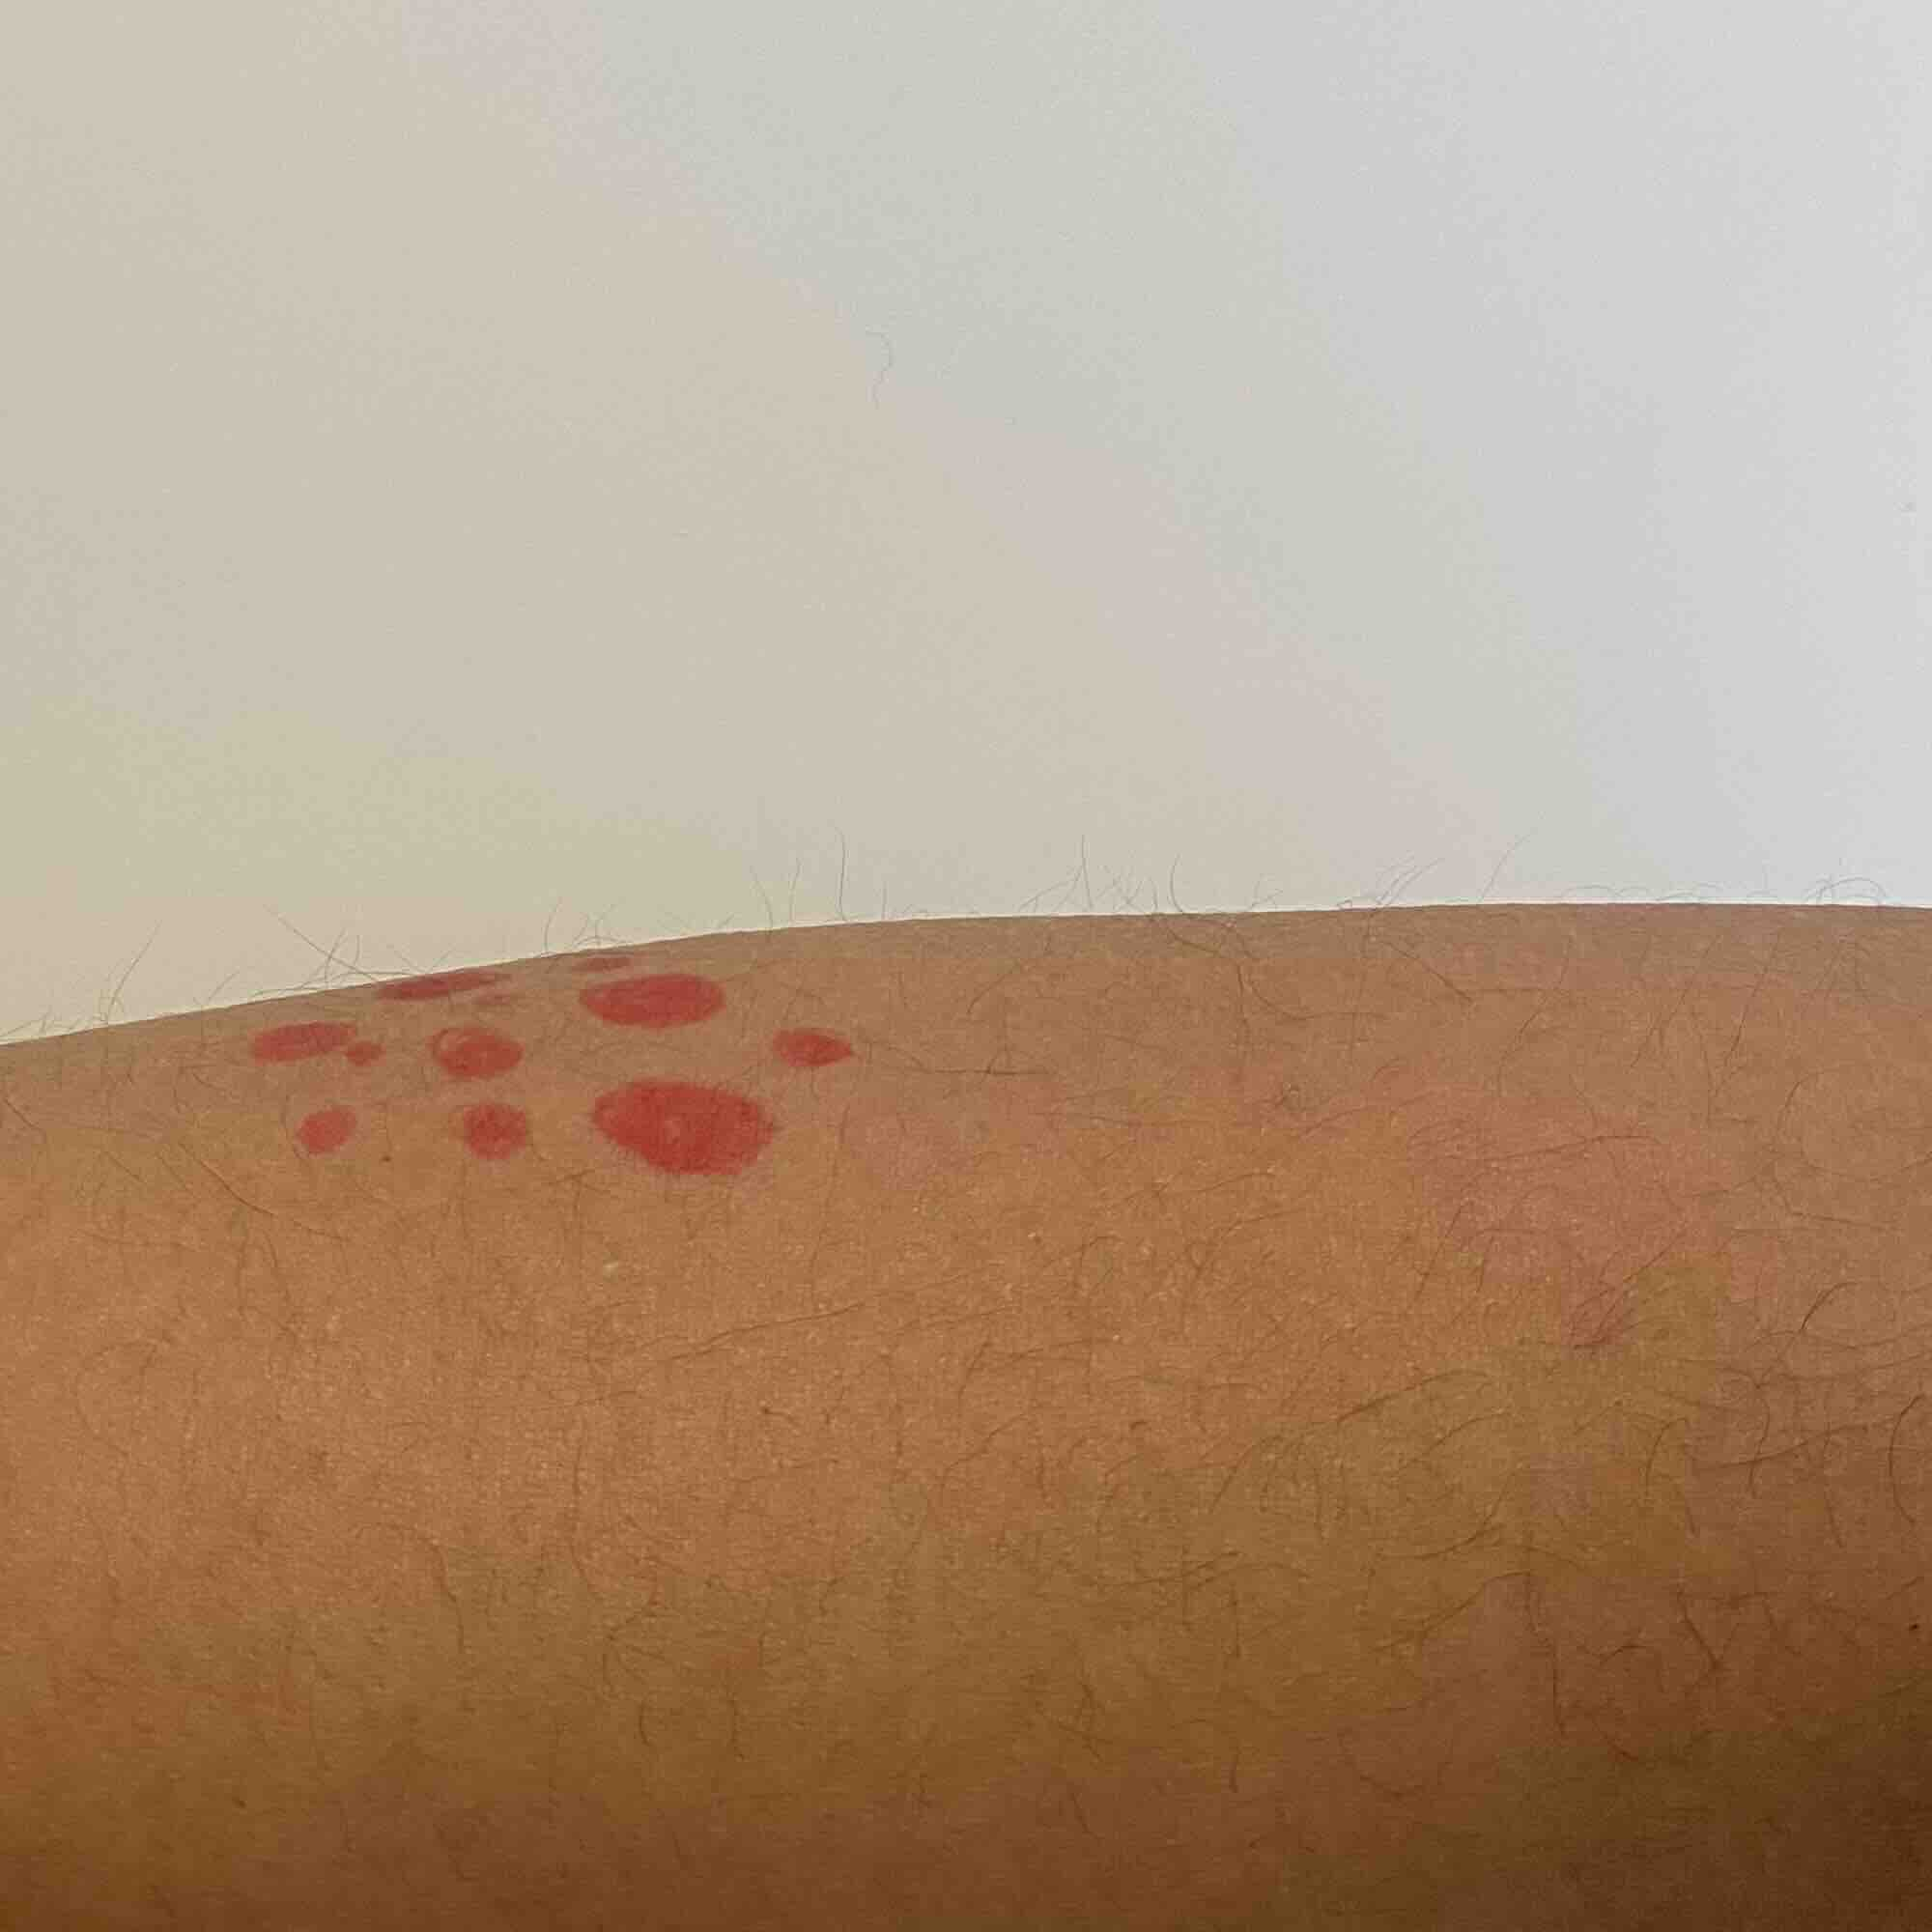
\includegraphics[width=\textwidth]{img/FoV.jpg}
        \caption{Field of View}
        \label{fig:FoV}
    \end{subfigure} 

    \begin{subfigure}[b]{0.24\textwidth}
        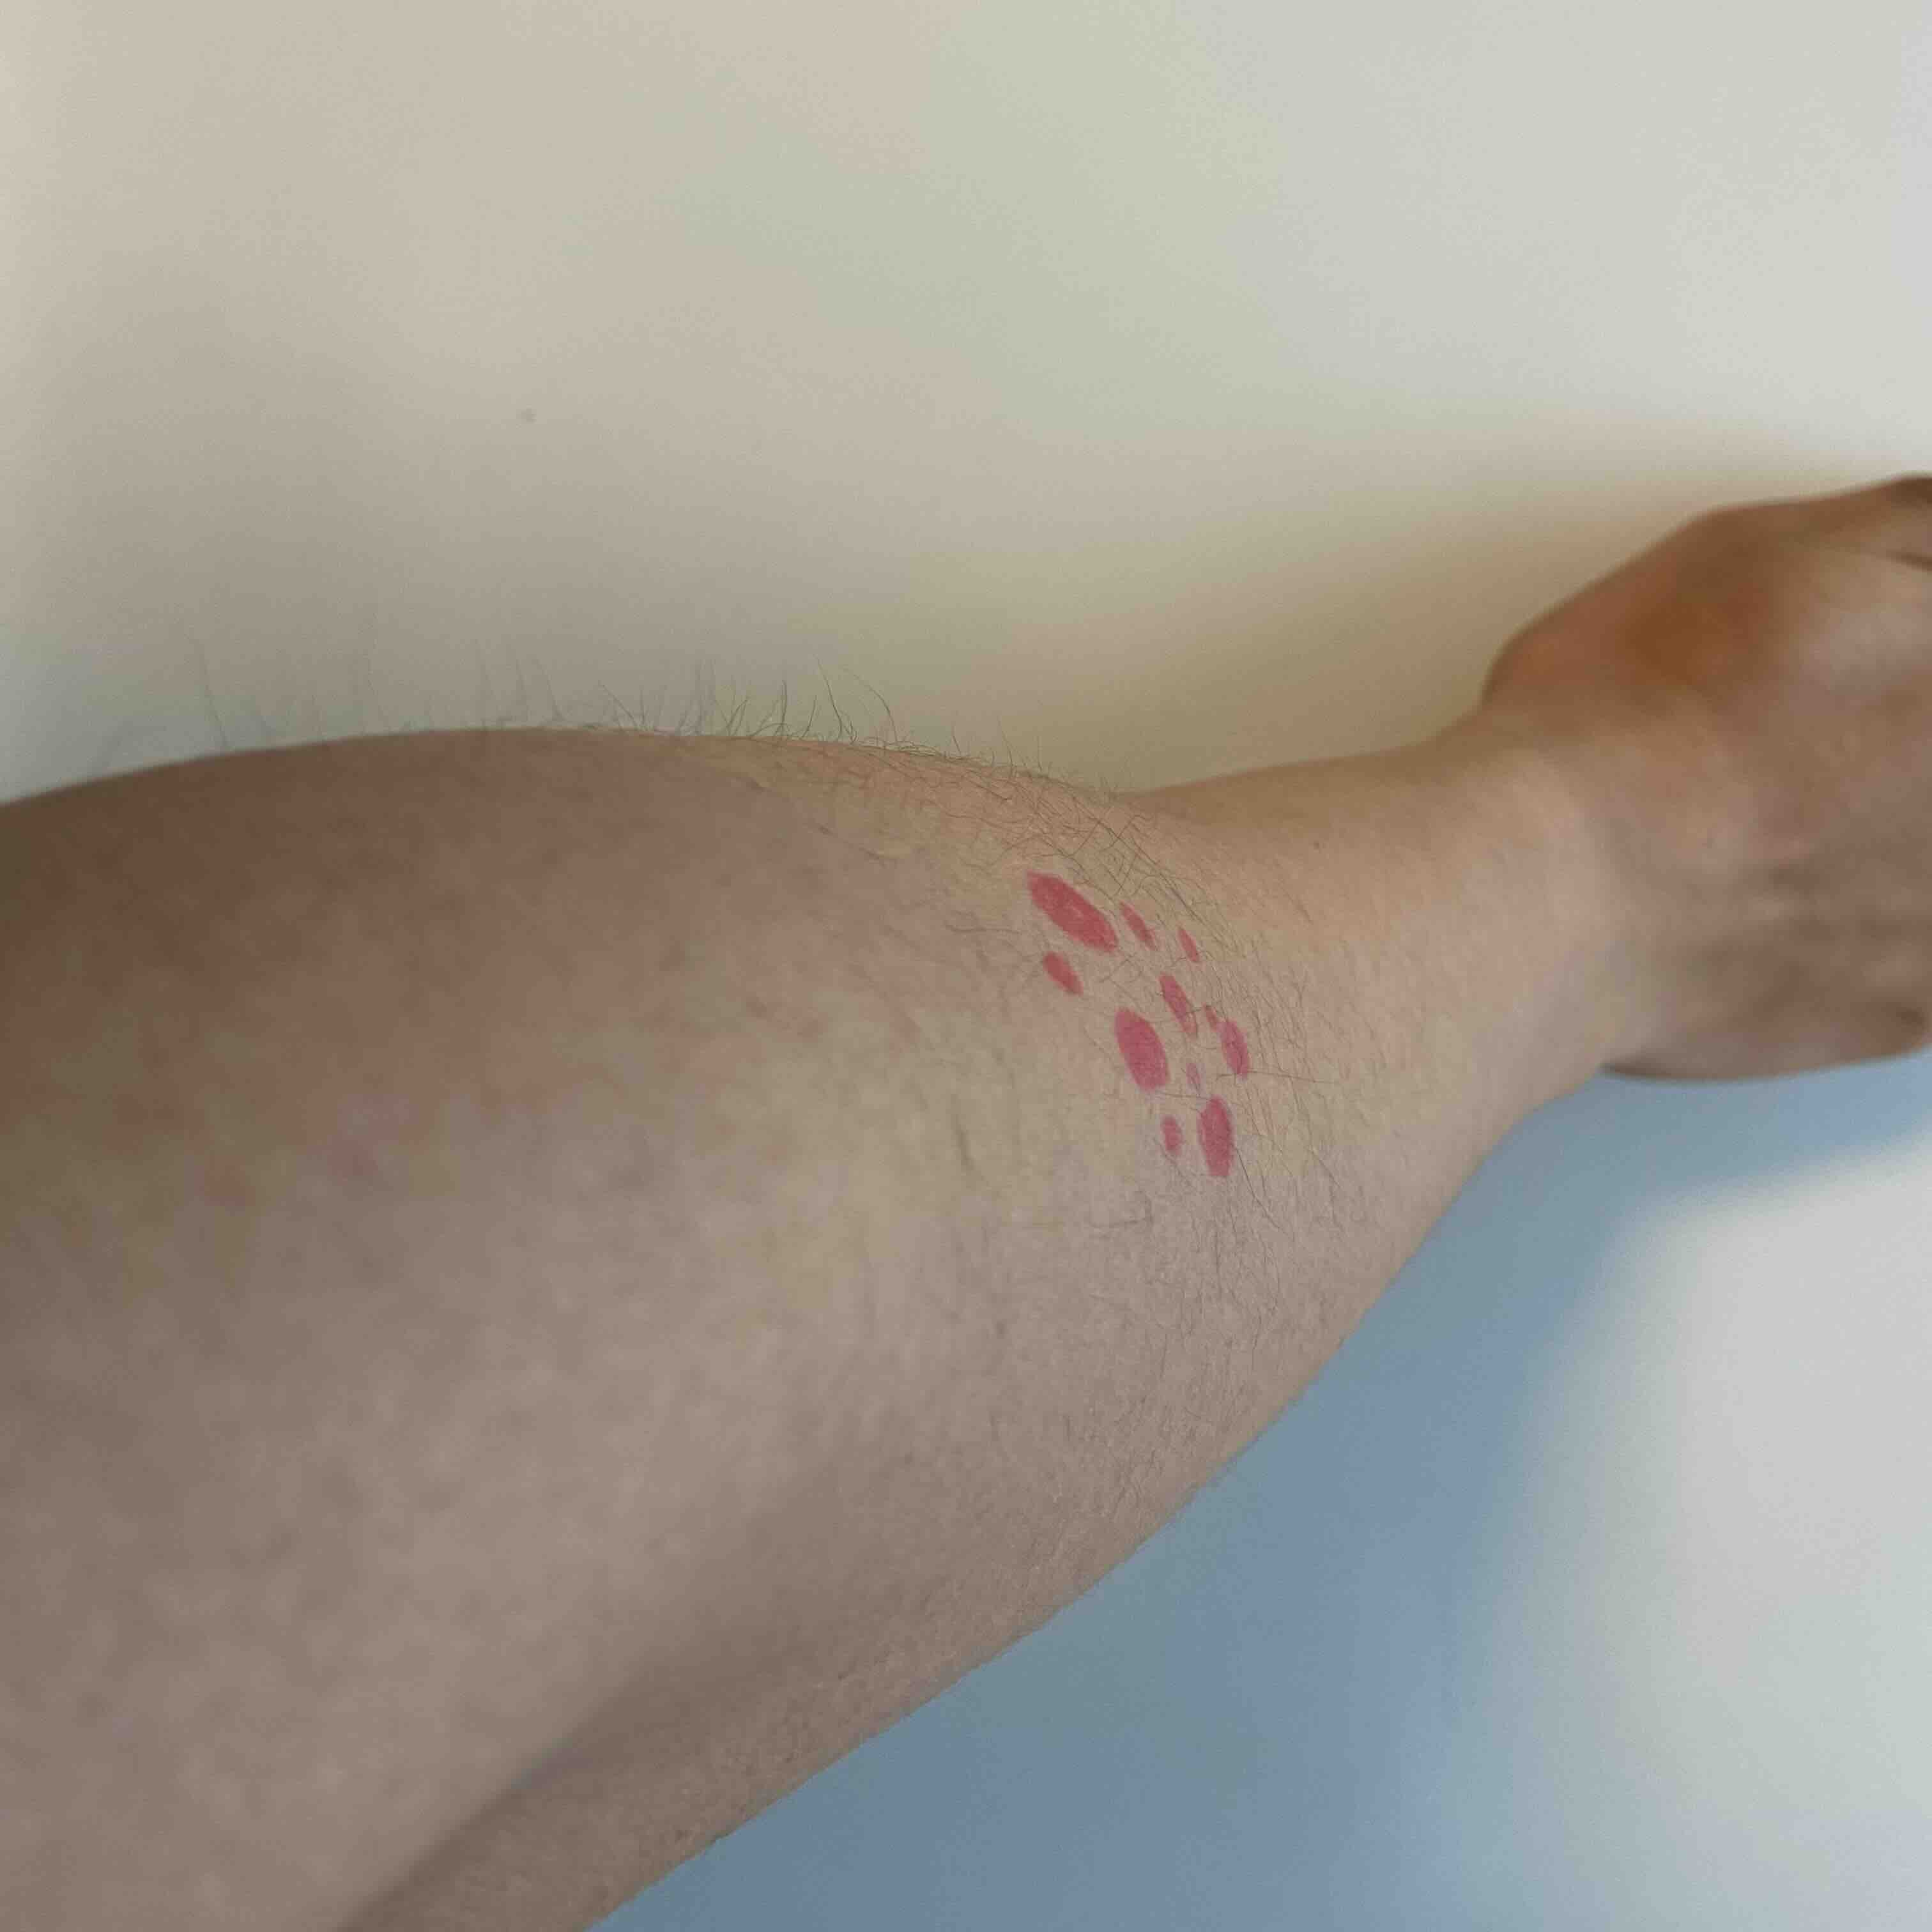
\includegraphics[width=\textwidth]{img/Orientation.jpg}
        \caption{Orientation}
        \label{fig:orientation}
    \end{subfigure}
    \hfill
    \begin{subfigure}[b]{0.24\textwidth}
        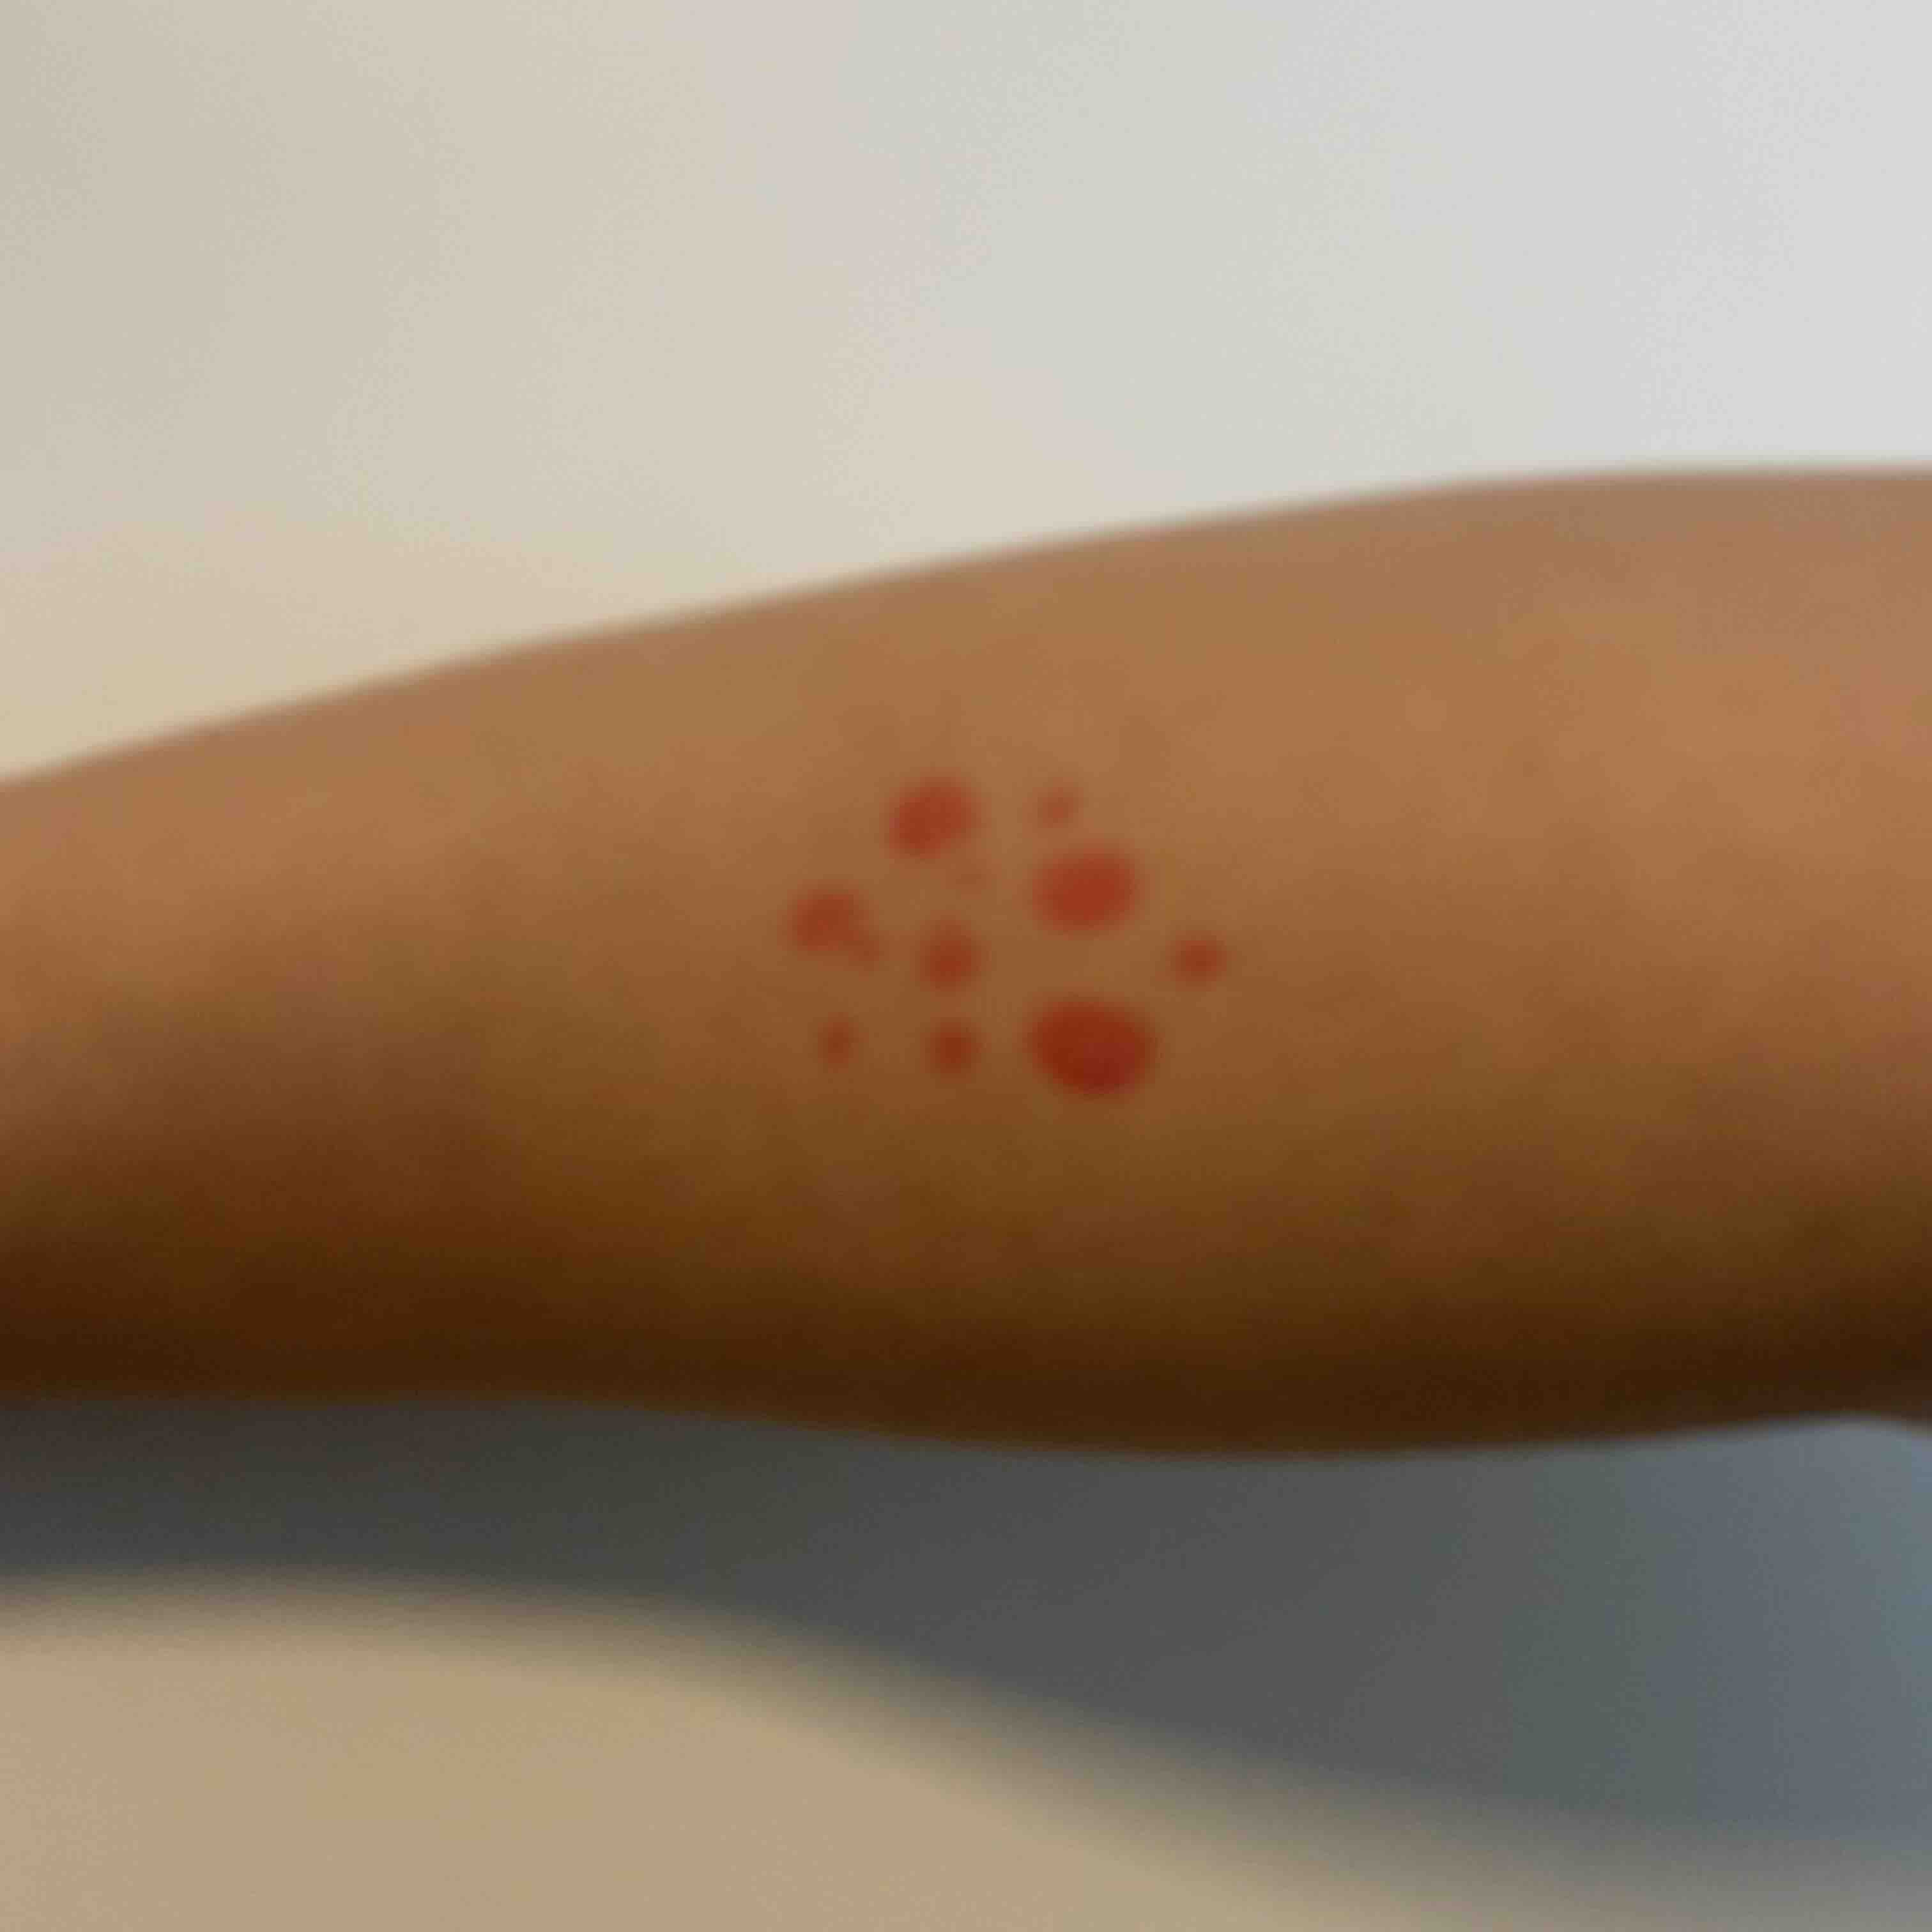
\includegraphics[width=\textwidth]{img/Focus.jpg}
        \caption{Focus}
        \label{fig:focus}
    \end{subfigure}
    \hfill
    \begin{subfigure}[b]{0.24\textwidth}
        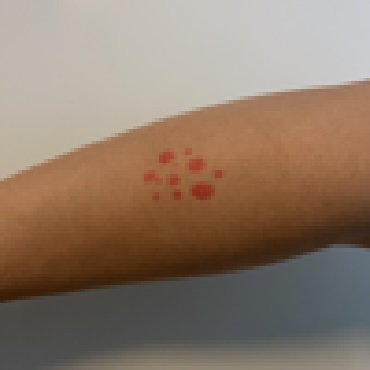
\includegraphics[width=\textwidth]{img/Resolution.jpg}
        \caption{Resolution}
        \label{fig:resol}
    \end{subfigure}
    \hfill
    \begin{subfigure}[b]{0.24\textwidth}
        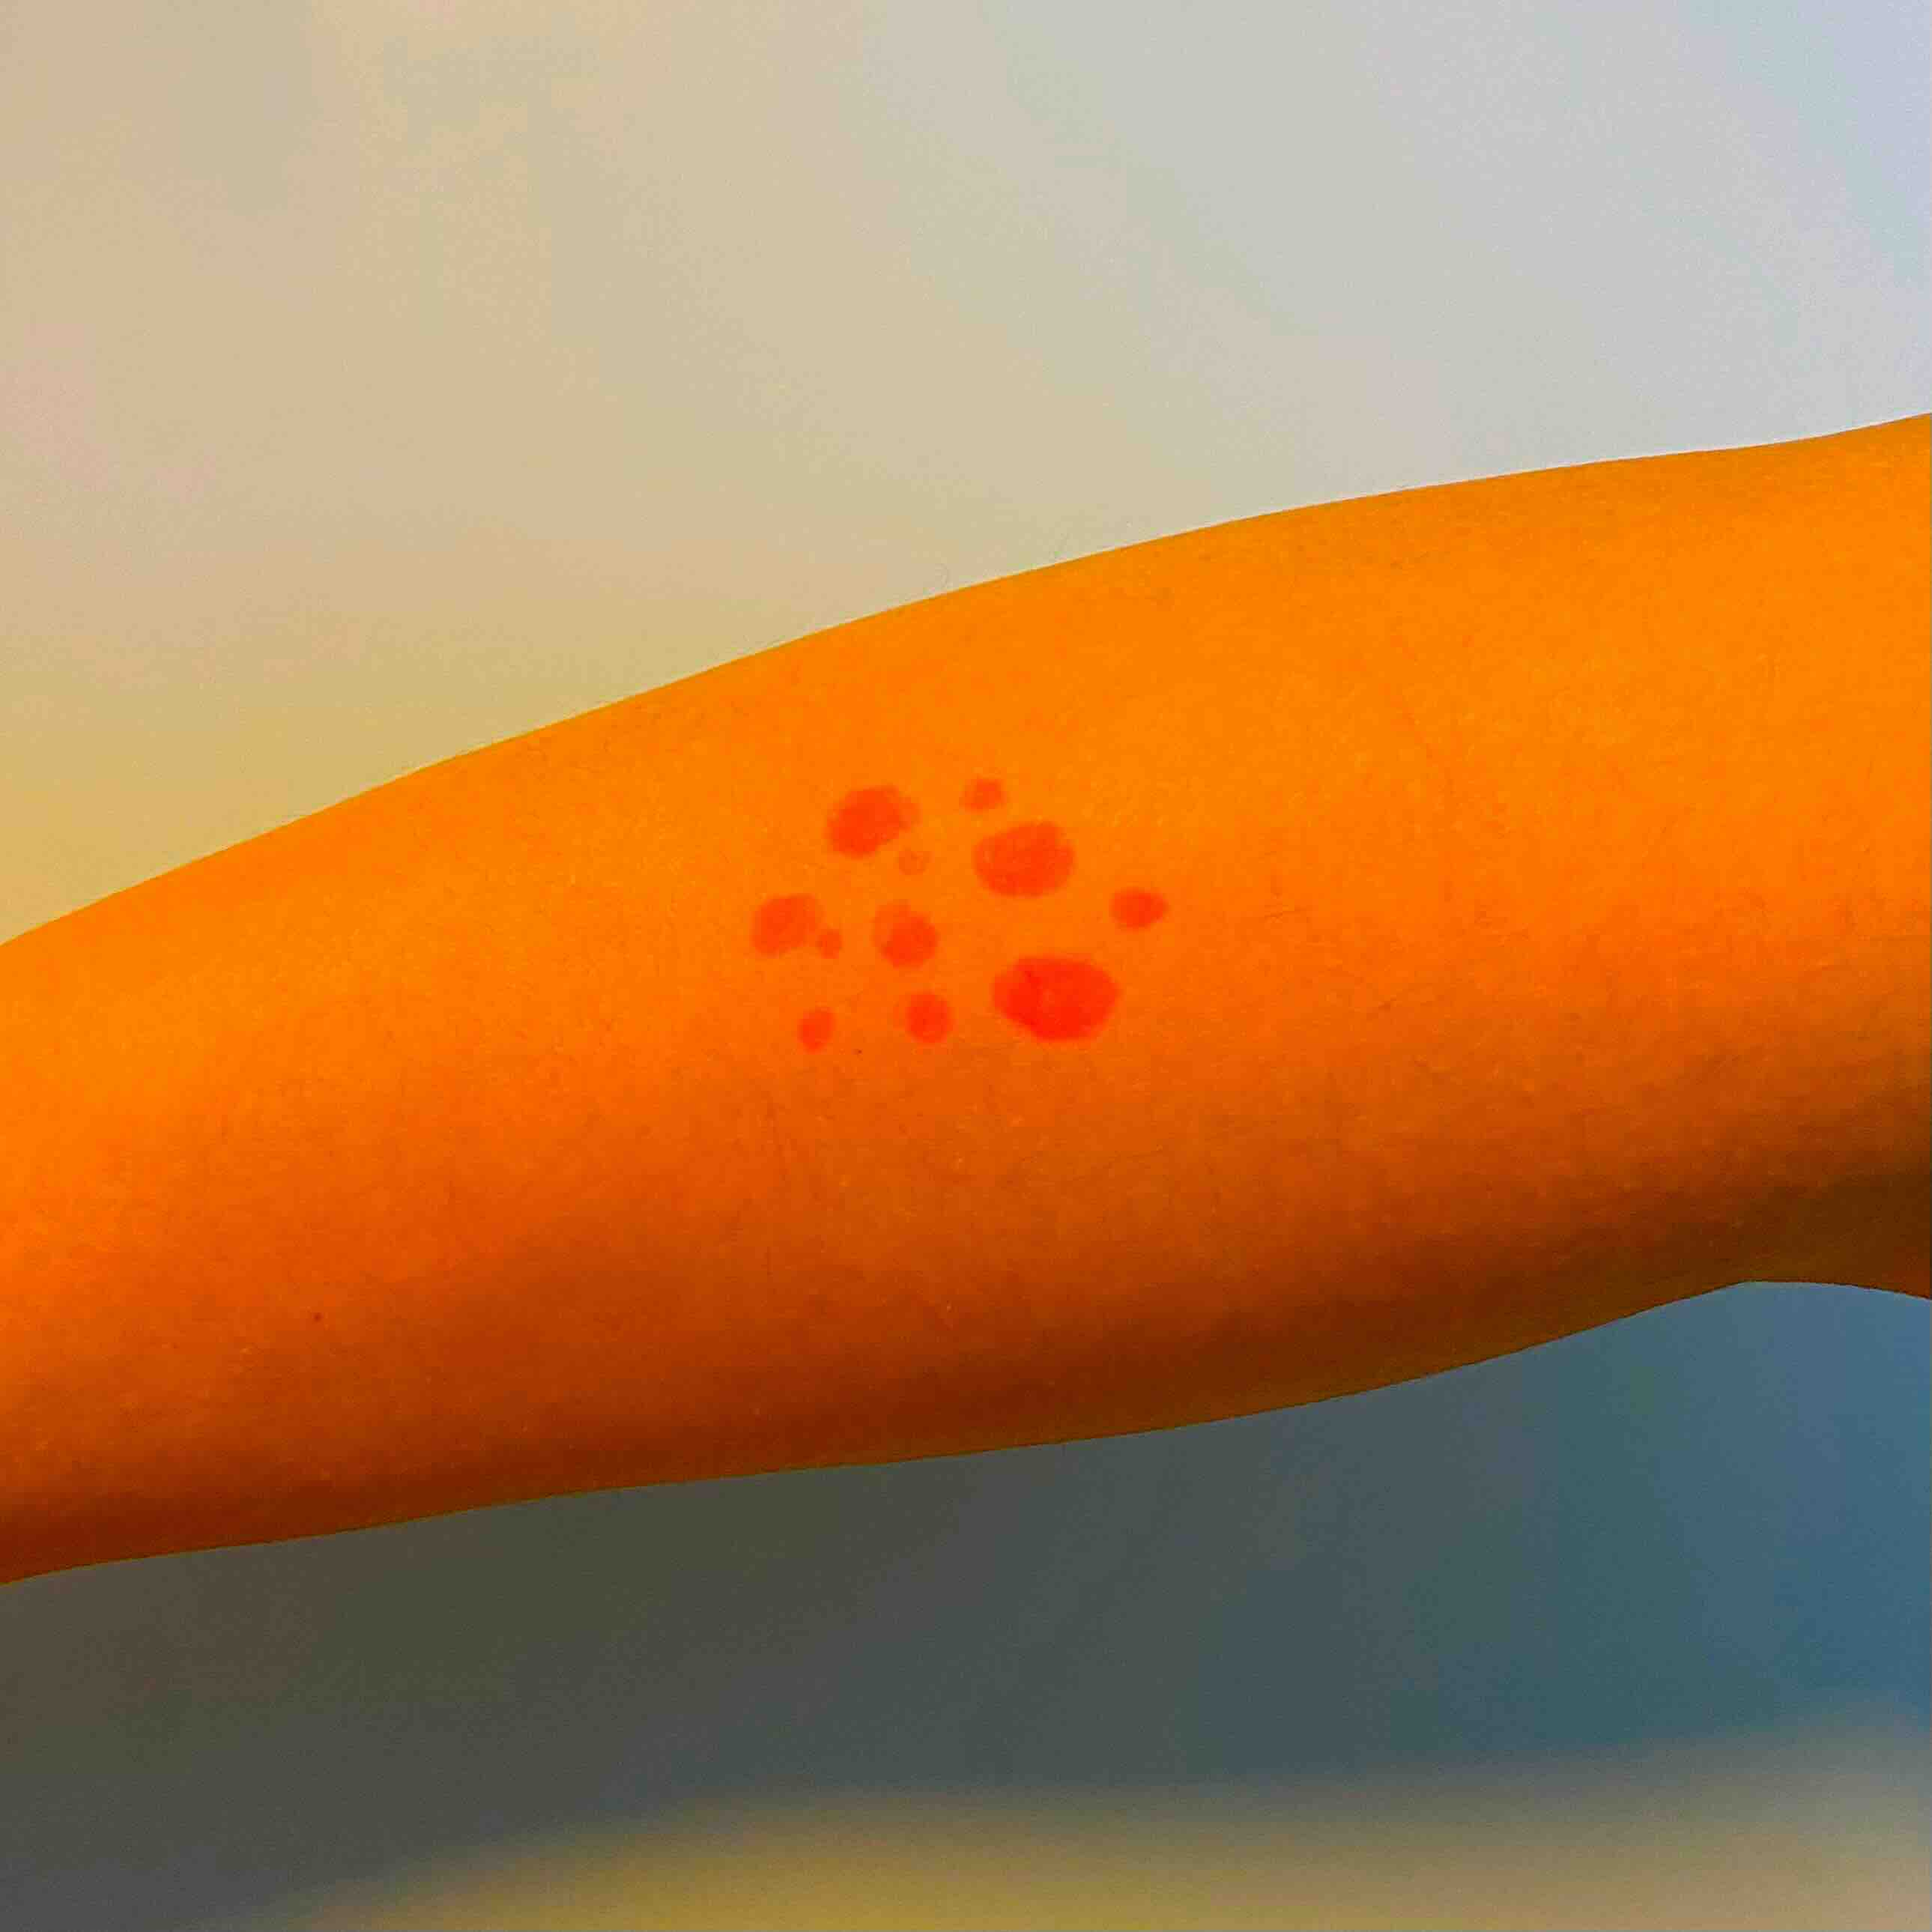
\includegraphics[width=\textwidth]{img/Color.jpg}
        \caption{Color Calibration}
        \label{fig:cc}
    \end{subfigure}
    \caption{Examples of teledermatology images showing good quality, poor lighting, distracting background, improper field of view, incorrect orientation, lack of focus, low resolution, and poor color calibration.}
    \label{fig:quality_criteria}
\end{figure}
\begin{enumerate}
    \item \textbf{Lighting}:  Good lighting is essential. It should be even and not too harsh, avoiding shadows or bright spots that can hide details. \textit{Use natural light or soft artificial light to clearly show the skin lesion.}
    \item \textbf{Background}:  The background should be plain and uncluttered to keep the focus on the skin issue. A simple, non-reflective background like white or gray works best. \textit{Use a plain, non-reflective background to minimize distractions and keep the focus on the skin lesion.}
    \item \textbf{Field of View}: The image should include the entire lesion and some surrounding skin. This helps provide context for a more accurate diagnosis. \textit{Make sure the lesion is centered and fully visible in the frame.}
    \item \textbf{Orientation}: The image should be taken from the correct angle to match standard anatomical positions. This helps the dermatologist understand where the lesion is on the body. \textit{Keep the camera straight and aligned with the lesion.}
    \item \textbf{Focus \& Depth of Field}: The image should be in sharp focus, with the entire lesion clear and detailed. Adjust the camera settings to ensure the lesion is not blurry. \textit{Ensure the camera is in focus and adjust the aperture to achieve sufficient depth of field.}
    \item \textbf{Resolution}: High resolution is important to show fine details. Use a camera with good resolution settings to capture clear and detailed images of the skin. \textit{Adjust the camera settings to the highest resolution possible to ensure clarity and precision in the image.}
    \item \textbf{Color Calibration}:  Accurate colors are necessary to assess the skin lesion correctly. Make sure the colors in the image match real life. \textit{Use a color reference chart or adjust the white balance settings on the camera to ensure accurate color reproduction.}
\end{enumerate}
By following these guidelines, teledermatology practitioners can ensure their images are of high quality, leading to better diagnoses and patient care.


\subsection{Teledermatology Datasets}
\label{sub:DatasetsTD}
In teledermatology, having high-quality image datasets is crucial for developing and testing methods to assess image quality. While many datasets exist for dermatology, they are not always designed specifically for teledermatology. The main difference is that dermatology datasets often include more professional images taken in clinical settings, including close-up dermoscopic images which provide detailed views of the skin. \par
\vspace{\baselineskip}
\noindent
Here are seven public datasets that can be used for teledermatology:
\begin{itemize}
    \item \textbf{ACNE04}: This dataset focuses on acne severity and lesion counting, containing 1,457 images with detailed annotations for training and testing purposes \autocite{ACNE04}.
    \item \textbf{DDI}: Provides 656 high-quality images curated by dermatologists for detailed skin tone evaluation and diagnostic accuracy \autocite{DDI}.
    \item \textbf{Derm7pt}: Utilizes 1,011 lesion cases to train a neural network for classifying skin lesions and melanoma using the 7-point checklist \autocite{Derm7pt}.
    \item \textbf{Fitzpatrick17k}: Includes 16,577 images annotated for Fitzpatrick skin type across 114 different skin conditions \autocite{F17K}.
    \item \textbf{Monkeypox Dataset 2022}: Contains approximately 1,905 images focused on monkeypox, useful for developing diagnostic tools \autocite{Monkeypox}.
    \item \textbf{PAD-UFES-20}: Comprises 2,298 clinical images from smartphones, enriched with clinical metadata for comprehensive research \autocite{PAD-UFES-20}.
    \item \textbf{SCIN}: Emerged from a crowdsourcing initiative, this dataset contains 10,408 images capturing a broad spectrum of dermatological conditions \autocite{SCIN}.
\end{itemize}
\noindent
These datasets provide valuable images and annotations that help develop and test image quality assessment methods for teledermatology. \par 

\subsection{Related Work on Image Quality Assessment in Teledermatology}
\label{sub:ApproachesIQAinTeledermatology}
In teledermatology, two key methods for detecting image quality have been highlighted in previous studies: TrueImage \autocite{TrueImage} and ImageQX \autocite{ImageQX}. Both methods work closely with dermatologists to ensure their models understand what is needed for accurate diagnoses. \par
\vspace{\baselineskip}
\noindent
\textbf{TrueImage} (A Machine Learning Algorithm to Improve the Quality of Telehealth Photos), introduced in 2021, uses an automated machine learning system to detect poor-quality dermatology photos and help patients take better images. This method was developed because many low-quality images submitted by patients disrupt the clinical workflow. TrueImage uses a semantic segmentation algorithm to identify skin areas, then generates features and classifies the quality. It focuses on common issues like blur, poor lighting, and zoom problems. TrueImage is efficient enough to run on older smartphones and is easy to understand, making it reliable across different skin tones. It was trained on a diverse dataset, including images from Google Images and Stanford Health Care. However, it has limitations: it cannot handle cases where only the background is blurry or poorly lit, it cannot detect framing issues, and it cannot discard images that do not contain skin \autocite{TrueImage}.\par
\vspace{\baselineskip}
\noindent
Released in January 2023, \textbf{ImageQX} (Explainable Image Quality Assessments in Teledermatological Photography)
is a convolutional neural network that automatically assesses the quality of dermatology images. It focuses on issues like bad framing, poor lighting, blur, low resolution, and distance problems. ImageQX was trained on 26,635 photos and validated on 9,874 photos, each annotated by up to 12 board-certified dermatologists. Its main innovation is providing explanations for poor quality, guiding patients on how to take better images. ImageQX is lightweight, only 15 MB, and can be easily used on mobile devices. It achieves a macro F1-score of 0.73, showing its effectiveness in real-world applications.  However, it has limitations in handling certain quality issues, like explaining blurry images, and relies heavily on dermatologist-annotated images, highlighting the need for a diverse and high-quality training dataset \autocite{ImageQX}.
\par
\vspace{\baselineskip}
\noindent
Both ImageQX and TrueImage make significant contributions to automated image quality assessment in teledermatology. They both address common issues like blur and poor lighting. ImageQX excels in providing detailed feedback on how to improve image quality, while TrueImage focuses on being computationally efficient and interpretable, making it suitable for older smartphones. From these methods, we learn the importance of lightweight models, providing actionable feedback to users, and using a diverse training dataset to ensure robustness. However, there is still room for improvement in handling complex lighting conditions and ensuring accurate zoom detection. \par

\subsection{Challenges and Opportunities in Image Quality Assessment for Teledermatology}
\label{sub:ChallengesOpportunitiesTeledermatology}
Teledermatology faces several challenges similar to those in \autoref{sub:ChallengesOpportunitiesIQA}. A major issue is the subjectivity of image quality assessment. Different dermatologists might have different opinions on what makes a good image, making standardization difficult. This variability can affect the accuracy of medical diagnoses since the quality of images is crucial. Common problems in teledermatology images include blurring, poor lighting, compression artifacts, and color issues. Each problem affects the image differently, making it hard to develop methods that handle all these issues well. Additionally, high-quality reference images are often unavailable, making it tough to evaluate the quality of patient-taken images accurately. Patients also use various devices and capture images under different conditions, adding to the complexity. \par
\vspace{\baselineskip}
\noindent
Despite these challenges, there are significant opportunities to improve teledermatology. Collaboration with dermatologists, as seen in methods like ImageQX and TrueImage, can improve IQA models by ensuring they meet the needs of medical professionals. These models can provide real-time, actionable feedback to patients on how to take better images, improving the quality of images submitted for remote consultations.